% !TeX program = xelatex

% !TeX spellcheck = en_US
% !TeX spellcheck = ru_RU

\documentclass[a4paper, 12pt]{article}

\usepackage[english, russian]{babel}
\usepackage[utf8]{inputenc}
\usepackage[T2A]{fontenc}

\usepackage{fontspec}
\setmainfont[Scale=1.167]{Times New Roman}

\usepackage{unicode-math}
\setmathfont[Scale=1.2]{Times New Roman}

\usepackage{mathtools}
\usepackage{amsmath, amsfonts, amsthm, physics, interval, bm}

\usepackage{indentfirst}
\usepackage{lipsum}
\usepackage{standalone}

\usepackage{algorithm2e}

\usepackage{pdflscape}
\usepackage{cancel}

\usepackage{tikz}
\usetikzlibrary{arrows.meta}

\usepackage[left=3cm, right=1.5cm, top=2cm, bottom=2cm]{geometry}

\usepackage{interval}
\usepackage{booktabs}
\usepackage{multirow}
\usepackage{makecell}

\usepackage{hyperref}

% \hypersetup{
%   linkcolor=blue,
%   urlcolor=cyan,
%   colorlinks=true,
%   linktoc=page,
% }

\usepackage{listings}
\usepackage{lstautogobble}

\lstset{
  language=Python,
  frame=tb,
  basicstyle=\scriptsize\ttfamily,
  commentstyle=\color{green},
  stringstyle=\color{red},
  tabsize=4,
  numbers=left,
  showstringspaces=false,
  keywordstyle=\color{blue},
  autogobble=true
}

\usepackage{adjustbox}

\usepackage{graphicx}
\usepackage{subcaption}
\usepackage{float}
\usepackage[font=small]{caption}

\usepackage[onehalfspacing]{setspace}
\setlength{\parindent}{1.25cm}
\setlength{\parskip}{0cm}

\addto\captionsrussian{\renewcommand{\contentsname}{\centering Содержание}}
% \renewcommand{\thesection}{}
% \renewcommand{\thesubsection}{\arabic{subsection}}

\sloppy


\begin{document}

  \renewcommand*{\vec}[1]{\mathbf{#1}}
  \newcommand{\Int}[2]{\int\limits_{#1}^{#2}}
  \newcommand{\Inner}[1]{\! #1 \,}
  \newcommand{\Dd}[1]{\dd #1}
  \newcommand{\Ddd}[2]{\dd #1 \dd #2}
  \newcommand{\MyVert}[1]{\Big\vert_{#1}}
  \newcommand{\MyVvert}[2]{\Big\vert_{\begin{subarray}{l} #1 \\ #2 \end{subarray}}}

  \newcommand{\Ttitle}[1]{\noindent\textbf{#1}}

  \tikzset{
  axes/.pic = {
    \draw[solid, thick, color=black, -{Stealth[scale=2]}] (0, 0) -- (40, 0);
    \draw[solid, thick, color=black, -{Stealth[scale=2]}] (0, 0) -- (0, 30);
    \node[scale=5] at (39, 2) {x};
    \node[scale=5] at (2, 29) {y};
  },
	grid/.pic = {
    \draw (0, 0) rectangle (32, 24);

    \draw (8, 0) -- (8, 24);
    \draw (16, 0) -- (16, 24);
    \draw (24, 0) -- (24, 24);

    \draw (0, 6) -- (32, 6);
    \draw (0, 12) -- (32, 12);
    \draw (0, 18) -- (32, 18);
  },
  inner/.pic = {
    \filldraw[red] (8, 6) circle (0.5);
    \filldraw[red] (16, 6) circle (0.5);
    \filldraw[red] (24, 6) circle (0.5);

    \filldraw[red] (8, 12) circle (0.5);
    \filldraw[red] (16, 12) circle (0.5);
    \filldraw[red] (24, 12) circle (0.5);

    \filldraw[red] (8, 18) circle (0.5);
    \filldraw[red] (16, 18) circle (0.5);
    \filldraw[red] (24, 18) circle (0.5);
  },
  left/.pic = {
    \filldraw[red] (0, 6) circle (0.5);
    \filldraw[red] (0, 12) circle (0.5);
    \filldraw[red] (0, 18) circle (0.5);
  },
  right/.pic = {
    \filldraw[red] (32, 6) circle (0.5);
    \filldraw[red] (32, 12) circle (0.5);
    \filldraw[red] (32, 18) circle (0.5);
  },
  bottom/.pic = {
    \filldraw[red] (8, 0) circle (0.5);
    \filldraw[red] (16, 0) circle (0.5);
    \filldraw[red] (24, 0) circle (0.5);
  },
  top/.pic = {
    \filldraw[red] (8, 24) circle (0.5);
    \filldraw[red] (16, 24) circle (0.5);
    \filldraw[red] (24, 24) circle (0.5);
  },
  leftbottom/.pic = {
    \filldraw[red] (0, 0) circle (0.5);
  },
  rightbottom/.pic = {
    \filldraw[red] (32, 0) circle (0.5);
  },
  righttop/.pic = {
    \filldraw[red] (32, 24) circle (0.5);
  },
  lefttop/.pic = {
    \filldraw[red] (0, 24) circle (0.5);
  },
}


  \begin{titlepage}

  \begin{center}
    Санкт-Петербургский политехнический университет Петра Великого\\
    Институт компьютерных наук и технологий\\
    Высшая школа программной инженерии\\[8cm]

    {\LARGE Курсовая работа}\\[0.5cm]
    \noindent\textbf{Разработка программного обеспечения для воспроизведения на ЭВМ двумерных стационарных моделей}\\[0.1cm]
    \noindent по дисциплине <<Математические модели>>\\[3cm]
  \end{center}

    \noindent Выполнил\\
    \noindent студент гр. 3530904/00104 \hfill В. Д. Яровой\\

    \noindent Проверил\\
    \noindent доцент, к. ф.-м. н. \hfill С. П. Воскобойников

  \vfill

  \begin{center}
    Санкт-Петербург\\
    \the\year
  \end{center}

\end{titlepage}

  \setcounter{page}{2}
  \tableofcontents

  \newpage
  \section*{Введение}\label{introduction}
  \addcontentsline{toc}{section}{\nameref{introduction}}
  \noindent Цель работы:
\begin{enumerate}
  \item Приобретение практического опыта в разработке программного обеспечения для задач моделирования двумерных
  стационарных процессов. В качестве примера выбраны процессы теплопроводности.
  \item Практическое построение дискретных моделей на основе интегро-интерполяционного метода.
  \item Практика в разработке тестовых примеров для отладки программ на основе метода пробных решений.
  \item Практика в использовании алгоритмического языка Фортран.
  \item Приобретение опыта представления результатов моделирования.
\end{enumerate}

\noindent Содержание работы:
\begin{enumerate}
  \item Изучение методов построения дискретных моделей для решения конкретной задачи.
  \item Написание программы на алгоритмическом языке и ее отладка.
  \item Решение с помощью разработанной программы конкретной задачи.
  \item Экспериментальное исследование точностных и временных характеристик разработанного программного обеспечения.
  \item Представление полученных результатов в виде таблиц и графиков.
\end{enumerate}


  % done
  \newpage
  \section{Постановка задачи}
  \textbf{Вариант В12.} Используя интегро-интерполяционный метод,
разработать программу для моделирования распределения температуры
в брусе, описываемого математической моделью
\begin{equation}\label{main-equation}
  - \left[
    \pdv{x} \left( k_1(x, y) \pdv{u}{x} \right) +
    \pdv{y} \left( k_2(x, y) \pdv{u}{y} \right)
  \right] = f(x, y)
\end{equation}
\[ a \leq x \leq b \]
\[ c \leq y \leq d \]
\[ 0 < c_{11} \leq k_1 \leq c_{12} \]
\[ 0 < c_{21} \leq k_2 \leq c_{22} \]
с граничными условиями
\begin{align*}
  u \MyVert{x = a} &= g_1(y)
  &
  - k_1 \pdv{u}{x}\MyVert{x = b} &= \chi_2 u \MyVert{x = b} - g_2(y) \\
  k_2 \pdv{u}{y}\MyVert{y = c} &= \chi_3 u \MyVert{y = c} - g_3(x)
  &
  - k_2 \pdv{u}{y}\MyVert{y = d} &= \chi_4 u \MyVert{y = d} - g_4(x)
\end{align*}
% Для решения системы линейных алгебраических уравнений использовать
% метод сопряженных градиентов с предобусловливанием. Матрица
% алгебраической системы должна храниться в упакованной форме -- сжатый
% разреженный строчный вид (4).


  \newpage
  \section{Использованное ПО}
  Программа для выполнения курсовой работы была написана на языке \href{https://www.python.org/}{Python}.
Список использованных сторонних библиотек приведен ниже.
\begin{itemize}
    \item \href{https://numpy.org/}{NumPy} -- базовый пакет для научных вычислений.
    \item \href{https://numpy.org/}{SymPy} -- пакет для символьных вычислений.
\end{itemize}

  \newpage
  \section{Вывод разностной схемы}
  В прямоугольнике $[a, b] \times [c, d]$ введем сетку с равномерным шагом $h_x$ и $h_y$.
\[ h_x = \frac{b - a}{N_x} \]
\[ h_y = \frac{d - c}{N_y} \]
где $N_x$ и $N_y$ -- число разбиений сетки. Тогда координаты узлов построенной сетки
вычисляются следуюим образом
\[ x_i = a + i h_x,\quad 0 \leq i \leq N_x \]
\[ y_j = c + j h_y,\quad 0 \leq j \leq N_y \]
Также введем вспомогательную сетку, координаты узлов которой вычисляются как
\[ x_{i+1/2} = \frac{x_{i+1} - x_i}{2},\quad 0 \leq i < N_x \]
\[ y_{j+1/2} = \frac{y_{j+1} - y_j}{2},\quad 0 \leq j < N_y \]
Теперь построим разностную схему в узлах основной сетки.

\subsection{Аппроксимация во внутрениих точках}
Проинтегрируем уравнение (\ref{main-equation}) во внутренних точках сетки.
\[
  - \left[
  \underbrace{ \Int{x_{i-1/2}}{x_{i+1/2}}\Int{y_{j-1/2}}{y_{j+1/2}} \Inner{\pdv{x}\left( k_1 \pdv{u}{x} \right)} \Ddd{x}{y} }_{I_1} +
  \underbrace{ \Int{x_{i-1/2}}{x_{i+1/2}}\Int{y_{j-1/2}}{y_{j+1/2}} \Inner{\pdv{y}\left( k_2 \pdv{u}{y} \right)} \Ddd{x}{y} }_{I_2}
  \right] =
  \underbrace{ \Int{x_{i-1/2}}{x_{i+1/2}}\Int{y_{j-1/2}}{y_{j+1/2}} \Inner{f} \Ddd{x}{y} }_{I_3}
\]
Проинтегрируем левую часть один раз.
\[ I_1 = \Int{y_{j-1/2}}{y_{j+1/2}} \Inner{k_1(x_{i+1/2},y) \pdv{u}{x} \MyVert{x = x_{i+1/2}}} \Dd{y} - \Int{y_{j-1/2}}{y_{j+1/2}} \Inner{k_1(x_{i-1/2},y) \pdv{u}{x} \MyVert{x = x_{i-1/2}}} \Dd{y} \]
\[ I_2 = \Int{x_{i-1/2}}{x_{i+1/2}} \Inner{k_2(x,y_{j+1/2}) \pdv{u}{y} \MyVert{y = y_{j+1/2}}} \Dd{x} - \Int{x_{i-1/2}}{x_{i+1/2}} \Inner{k_2(x,y_{j-1/2}) \pdv{u}{y} \MyVert{y = y_{j-1/2}}} \Dd{x} \]
Найдем интегралы с помощью формулы средних прямоугольников.
\[ I_1 \approx h_y k_1(x_{i+1/2},y_{j}) \pdv{u}{x} \MyVvert{x = x_{i+1/2}}{y = y_{j}} - h_y k_1(x_{i-1/2},y_{j}) \pdv{u}{x} \MyVvert{x = x_{i-1/2}}{y = y_{j}} \]
\[ I_2 \approx h_x k_2(x_{i},y_{j+1/2}) \pdv{u}{y} \MyVvert{x = x_{i}}{y = y_{j+1/2}} - h_x k_2(x_{i},y_{j-1/2}) \pdv{u}{y} \MyVvert{x = x_{i}}{y = y_{j-1/2}} \]
Теперь воспользуемся формулами численного дифференцирования.
\[ I_1 \approx h_y k_1(x_{i+1/2},y_{j}) \frac{v_{i+1,j} - v_{i,j}}{h_x} - h_y k_1(x_{i-1/2},y_{j}) \frac{v_{i,j} - v_{i-1,j}}{h_x} \]
\[ I_2 \approx h_x k_2(x_{i},y_{j+1/2}) \frac{v_{i,j+1} - v_{i,j}}{h_y} - h_x k_2(x_{i},y_{j-1/2}) \frac{v_{i,j} - v_{i,j-1}}{h_y} \]
Также с помощью формулы средних прямоугольников найдем интеграл в правой части.
\[ I_3 \approx h_x h_y f_{i,j} \]
Получим уравнение разностной схемы для $i = \overline{1,N_x-1}$ и $j = \overline{1,N_y-1}$.
\begin{multline*}
  - \left[
  h_y k_1(x_{i+1/2},y_{j}) \frac{v_{i+1,j} - v_{i,j}}{h_x} - h_y k_1(x_{i-1/2},y_{j}) \frac{v_{i,j} - v_{i-1,j}}{h_x} + \right. \\
  \left. +
  h_x k_2(x_{i},y_{j+1/2}) \frac{v_{i,j+1} - v_{i,j}}{h_y} - h_x k_2(x_{i},y_{j-1/2}) \frac{v_{i,j} - v_{i,j-1}}{h_y}
  \right] =
  h_x h_y f_{i,j}
\end{multline*}

\subsection{Аппроксимация на левой границе}
Проинтегрируем уравнение (\ref{main-equation}) на левой границе сетки.
\[
  - \left[
  \underbrace{ \Int{x_{0}}{x_{1/2}}\Int{y_{j-1/2}}{y_{j+1/2}} \Inner{\pdv{x}\left( k_1 \pdv{u}{x} \right)} \Ddd{x}{y} }_{I_1} +
  \underbrace{ \Int{x_{0}}{x_{1/2}}\Int{y_{j-1/2}}{y_{j+1/2}} \Inner{\pdv{y}\left( k_2 \pdv{u}{y} \right)} \Ddd{x}{y} }_{I_2}
  \right] =
  \underbrace{ \Int{x_{0}}{x_{1/2}}\Int{y_{j-1/2}}{y_{j+1/2}} \Inner{f} \Ddd{x}{y} }_{I_3}
\]
Проинтегрируем левую часть один раз.
\[ I_1 = \Int{y_{j-1/2}}{y_{j+1/2}} \Inner{k_1(x_{1/2},y) \pdv{u}{x} \MyVert{x = x_{1/2}}} \Dd{y} - \Int{y_{j-1/2}}{y_{j+1/2}} \Inner{k_1(x_{0},y) \pdv{u}{x} \MyVert{x = x_{0}}} \Dd{y} \]
\[ I_2 = \Int{x_{0}}{x_{1/2}} \Inner{k_2(x,y_{j+1/2}) \pdv{u}{y} \MyVert{y = y_{j+1/2}}} \Dd{x} - \Int{x_{0}}{x_{1/2}} \Inner{k_2(x,y_{j-1/2}) \pdv{u}{y} \MyVert{y = y_{j-1/2}}} \Dd{x} \]
Найдем интегралы с помощью формулы левых прямоугольников.
\[ I_1 \approx h_y k_1(x_{1/2},y_{j}) \pdv{u}{x} \MyVvert{x = x_{1/2}}{y = y_{j}} - h_y k_1(x_{0},y_{j}) \pdv{u}{x} \MyVvert{x = x_{0}}{y = y_{j}} \]
\[ I_2 \approx \frac{h_x}{2} k_2(x_{0},y_{j+1/2}) \pdv{u}{y} \MyVvert{x = x_{0}}{y = y_{j+1/2}} - \frac{h_x}{2} k_2(x_{0},y_{j-1/2}) \pdv{u}{y} \MyVvert{x = x_{0}}{y = y_{j-1/2}} \]
Теперь воспользуемся формулами численного дифференцирования и известным граничным условием.
\[ I_1 \approx h_y k_1(x_{1/2},y_{j}) \frac{v_{1,j} - v_{0,j}}{h_x} - h_y \left( \chi_1 v_{0,j} - g_1(y_{j}) \right) \]
\[ I_2 \approx \frac{h_x}{2} k_2(x_{0},y_{j+1/2}) \frac{v_{0,j+1} - v_{0,j}}{h_y} - \frac{h_x}{2} k_2(x_{0},y_{j-1/2}) \frac{v_{0,j} - v_{0,j-1}}{h_y} \]
Также с помощью формул средних и левых прямоугольников найдем интеграл в правой части.
\[ I_3 \approx \frac{h_x}{2} h_y f_{0,j} \]
Получим уравнение разностной схемы для $i = 0$ и $j = \overline{1,N_y-1}$.
\begin{multline*}
  - \left[
  h_y k_1(x_{1/2},y_{j}) \frac{v_{1,j} - v_{0,j}}{h_x} - h_y \left( \chi_1 v_{0,j} - g_1(y_{j}) \right) + \right. \\
  \left. +
  \frac{h_x}{2} k_2(x_{0},y_{j+1/2}) \frac{v_{0,j+1} - v_{0,j}}{h_y} - \frac{h_x}{2} k_2(x_{0},y_{j-1/2}) \frac{v_{0,j} - v_{0,j-1}}{h_y}
  \right] =
  \frac{h_x}{2} h_y f_{0,j}
\end{multline*}

\subsection{Аппроксимация на правой границе}
В качестве уравнения разностной схемы для $i = N_x$ и $j = \overline{1,N_y-1}$ возьмем
известное граничное условие.
\[ u \MyVert{x = b} = g_2(y) \]
\[ v_{N_x,j} = g_2(y_j) \]

\subsection{Аппроксимация на нижней границе}
Проинтегрируем уравнение (\ref{main-equation}) на нижней границе сетки.
\[
  - \left[
  \underbrace{ \Int{x_{i-1/2}}{x_{i+1/2}}\Int{y_{0}}{y_{1/2}} \Inner{\pdv{x}\left( k_1 \pdv{u}{x} \right)} \Ddd{x}{y} }_{I_1} +
  \underbrace{ \Int{x_{i-1/2}}{x_{i+1/2}}\Int{y_{0}}{y_{1/2}} \Inner{\pdv{y}\left( k_2 \pdv{u}{y} \right)} \Ddd{x}{y} }_{I_2}
  \right] =
  \underbrace{ \Int{x_{i-1/2}}{x_{i+1/2}}\Int{y_{0}}{y_{1/2}} \Inner{f} \Ddd{x}{y} }_{I_3}
\]
Проинтегрируем левую часть один раз.
\[ I_1 = \Int{y_{0}}{y_{1/2}} \Inner{k_1(x_{i+1/2},y) \pdv{u}{x} \MyVert{x = x_{i+1/2}}} \Dd{y} - \Int{y_{0}}{y_{1/2}} \Inner{k_1(x_{i-1/2},y) \pdv{u}{x} \MyVert{x = x_{i-1/2}}} \Dd{y} \]
\[ I_2 = \Int{x_{i-1/2}}{x_{i+1/2}} \Inner{k_2(x,y_{1/2}) \pdv{u}{y} \MyVert{y = y_{1/2}}} \Dd{x} - \Int{x_{i-1/2}}{x_{i+1/2}} \Inner{k_2(x,y_{0}) \pdv{u}{y} \MyVert{y = y_{0}}} \Dd{x} \]
Найдем интегралы с помощью формулы левых прямоугольников.
\[ I_1 \approx \frac{h_y}{2} k_1(x_{i+1/2},y_0) \pdv{u}{x} \MyVvert{x = x_{i+1/2}}{y = y_{0}} - \frac{h_y}{2} k_1(x_{i-1/2},y_0) \pdv{u}{x} \MyVvert{x = x_{i-1/2}}{y = y_{0}} \]
\[ I_2 \approx h_x k_2(x_i,y_{1/2}) \pdv{u}{y} \MyVvert{x = x_{i}}{y = y_{1/2}} - h_x k_2(x_i,y_{0}) \pdv{u}{y} \MyVvert{x = x_{i}}{y = y_{0}} \]
Теперь воспользуемся формулами численного дифференцирования и известным граничным условием.
\[ I_1 \approx \frac{h_y}{2} k_1(x_{i+1/2},y_0) \frac{v_{i+1,0} - v_{i,0}}{h_x} - \frac{h_y}{2} k_1(x_{i-1/2},y_0) \frac{v_{i,0} - v_{i-1,0}}{h_x} \]
\[ I_2 \approx h_x k_2(x_i,y_{1/2}) \frac{v_{i,1} - v_{i,0}}{h_y} - h_x \left( \chi_3 v_{i,0} - g_3(x_i) \right) \]
Также с помощью формул средних и левых прямоугольников найдем интеграл в правой части.
\[ I_3 \approx h_x \frac{h_y}{2} f_{i,0} \]
Получим уравнение разностной схемы для $i = \overline{1,N_x-1}$ и $j = 0$.
\begin{multline*}
  - \left[
  \frac{h_y}{2} k_1(x_{i+1/2},y_0) \frac{v_{i+1,0} - v_{i,0}}{h_x} - \frac{h_y}{2} k_1(x_{i-1/2},y_0) \frac{v_{i,0} - v_{i-1,0}}{h_x} + \right. \\
  \left. +
  h_x k_2(x_i,y_{1/2}) \frac{v_{i,1} - v_{i,0}}{h_y} - h_x \left( \chi_3 v_{i,0} - g_3(x_i) \right)
  \right] =
  h_x \frac{h_y}{2} f_{i,0}
\end{multline*}

\subsection{Аппроксимация на верхней границе}
Проинтегрируем уравнение (\ref{main-equation}) на верхней границе сетки.
\[
  - \left[
  \underbrace{ \Int{x_{i-1/2}}{x_{i+1/2}}\Int{y_{N_y-1/2}}{y_{N_y}} \Inner{\pdv{x}\left( k_1 \pdv{u}{x} \right)} \Ddd{x}{y} }_{I_1} +
  \underbrace{ \Int{x_{i-1/2}}{x_{i+1/2}}\Int{y_{N_y-1/2}}{y_{N_y}} \Inner{\pdv{y}\left( k_2 \pdv{u}{y} \right)} \Ddd{x}{y} }_{I_2}
  \right] =
  \underbrace{ \Int{x_{i-1/2}}{x_{i+1/2}}\Int{y_{N_y-1/2}}{y_{N_y}} \Inner{f} \Ddd{x}{y} }_{I_3}
\]
Проинтегрируем левую часть один раз.
\[ I_1 = \Int{y_{N_y-1/2}}{y_{N_y}} \Inner{k_1(x_{i+1/2},y) \pdv{u}{x} \MyVert{x = x_{i+1/2}}} \Dd{y} - \Int{y_{N_y-1/2}}{y_{N_y}} \Inner{k_1(x_{i-1/2},y) \pdv{u}{x} \MyVert{x = x_{i-1/2}}} \Dd{y} \]
\[ I_2 = \Int{x_{i-1/2}}{x_{i+1/2}} \Inner{k_2(x,y_{N_y}) \pdv{u}{y} \MyVert{y = y_{N_y}}} \Dd{x} - \Int{x_{i-1/2}}{x_{i+1/2}} \Inner{k_2(x,y_{N_y-1/2}) \pdv{u}{y} \MyVert{y = y_{N_y-1/2}}} \Dd{x} \]
Найдем интегралы с помощью формулы правых прямоугольников.
\[ I_1 \approx \frac{h_y}{2} k_1(x_{i+1/2},y_{N_y}) \pdv{u}{x} \MyVvert{x = x_{i+1/2}}{y = y_{N_y}} - \frac{h_y}{2} k_1(x_{i-1/2},y_{N_y}) \pdv{u}{x} \MyVvert{x = x_{i-1/2}}{y = y_{N_y}} \]
\[ I_2 \approx h_x k_2(x_i,y_{N_y}) \pdv{u}{y} \MyVvert{x = x_{i}}{y = y_{N_y}} - h_x k_2(x_i,y_{N_y-1/2}) \pdv{u}{y} \MyVvert{x = x_{i}}{y = y_{N_y-1/2}} \]
Теперь воспользуемся формулами численного дифференцирования и известным граничным условием.
\[ I_1 \approx \frac{h_y}{2} k_1(x_{i+1/2},y_{N_y}) \frac{v_{i+1,N_y} - v_{i,N_y}}{h_x} - \frac{h_y}{2} k_1(x_{i-1/2},y_{N_y}) \frac{v_{i,N_y} - v_{i-1,N_y}}{h_x} \]
\[ I_2 \approx h_x \left( - \chi_4 v_{i,N_y} + g_4(x_i) \right) - h_x k_2(x_i,y_{N_y-1/2}) \frac{v_{i,N_y} - v_{i,N_y-1}}{h_y} \]
Также с помощью формул средних и правых прямоугольников найдем интеграл в правой части.
\[ I_3 \approx h_x \frac{h_y}{2} f_{i,N_y} \]
Получим уравнение разностной схемы для $i = \overline{1,N_x-1}$ и $j = N_y$.
\begin{multline*}
  - \left[
  \frac{h_y}{2} k_1(x_{i+1/2},y_{N_y}) \frac{v_{i+1,N_y} - v_{i,N_y}}{h_x} - \frac{h_y}{2} k_1(x_{i-1/2},y_{N_y}) \frac{v_{i,N_y} - v_{i-1,N_y}}{h_x} + \right. \\
  \left. +
  h_x \left( - \chi_4 v_{i,N_y} + g_4(x_i) \right) - h_x k_2(x_i,y_{N_y-1/2}) \frac{v_{i,N_y} - v_{i,N_y-1}}{h_y}
  \right] =
  h_x \frac{h_y}{2} f_{i,N_y}
\end{multline*}

\subsection{Аппроксимация в левой нижней граничной точке}
Проинтегрируем уравнение (\ref{main-equation}) в левой нижней граничной точке сетки.
\[
  - \left[
  \underbrace{ \Int{x_{0}}{x_{1/2}}\Int{y_{0}}{y_{1/2}} \Inner{\pdv{x}\left( k_1 \pdv{u}{x} \right)} \Ddd{x}{y} }_{I_1} +
  \underbrace{ \Int{x_{0}}{x_{1/2}}\Int{y_{0}}{y_{1/2}} \Inner{\pdv{y}\left( k_2 \pdv{u}{y} \right)} \Ddd{x}{y} }_{I_2}
  \right] =
  \underbrace{ \Int{x_{0}}{x_{1/2}}\Int{y_{0}}{y_{1/2}} \Inner{f} \Ddd{x}{y} }_{I_3}
\]
Проинтегрируем левую часть один раз.
\[ I_1 = \Int{y_{0}}{y_{1/2}} \Inner{k_1(x_{1/2},y) \pdv{u}{x} \MyVert{x = x_{1/2}}} \Dd{y} - \Int{y_{0}}{y_{1/2}} \Inner{k_1(x_{0},y) \pdv{u}{x} \MyVert{x = x_{0}}} \Dd{y} \]
\[ I_2 = \Int{x_{0}}{x_{1/2}} \Inner{k_2(x,y_{1/2}) \pdv{u}{y} \MyVert{y = y_{1/2}}} \Dd{x} - \Int{x_{0}}{x_{1/2}} \Inner{k_2(x,y_{0}) \pdv{u}{y} \MyVert{y = y_{0}}} \Dd{x} \]
Найдем интегралы с помощью формулы левых прямоугольников.
\[ I_1 \approx \frac{h_y}{2} k_1(x_{1/2},y_{0}) \pdv{u}{x} \MyVvert{x = x_{1/2}}{y = y_{0}} - \frac{h_y}{2} k_1(x_{0},y_{0}) \pdv{u}{x} \MyVvert{x = x_{0}}{y = y_{0}} \]
\[ I_2 \approx \frac{h_x}{2}  k_2(x_{0},y_{1/2}) \pdv{u}{y} \MyVvert{x = x_{0}}{y = y_{1/2}} - \frac{h_x}{2}  k_2(x_{0},y_{0}) \pdv{u}{y} \MyVvert{x = x_{0}}{y = y_{0}} \]
Теперь воспользуемся формулами численного дифференцирования и известными граничными условиями.
\[ I_1 \approx \frac{h_y}{2}  k_1(x_{1/2},y_{0}) \frac{v_{1,0} - v_{0,0}}{h_x} - \frac{h_y}{2} \left( \chi_1 v_{0,0} - g_1(y_{0}) \right) \]
\[ I_2 \approx \frac{h_x}{2}  k_2(x_{0},y_{1/2}) \frac{v_{0,1} - v_{0,0}}{h_y} - \frac{h_x}{2} \left( \chi_3 v_{0,0} - g_3(x_{0}) \right) \]
Также с помощью формулы левых прямоугольников найдем интеграл в правой части.
\[ I_3 \approx \frac{h_x}{2} \frac{h_y}{2} f_{0,0} \]
Получим уравнение разностной схемы для $i = 0$ и $j = 0$.
\begin{multline*}
  - \left[
  \frac{h_y}{2}  k_1(x_{1/2},y_{0}) \frac{v_{1,0} - v_{0,0}}{h_x} - \frac{h_y}{2} \left( \chi_1 v_{0,0} - g_1(y_{0}) \right) + \right. \\
  \left. +
  \frac{h_x}{2}  k_2(x_{0},y_{1/2}) \frac{v_{0,1} - v_{0,0}}{h_y} - \frac{h_x}{2} \left( \chi_3 v_{0,0} - g_3(x_{0}) \right)
  \right] =
  \frac{h_x}{2} \frac{h_y}{2} f_{0,0}
\end{multline*}

\subsection{Аппроксимация в правой нижней граничной точке}
В качестве уравнения разностной схемы для $i = N_x$ и $j = 0$ возьмем
известное граничное условие.
\[ u \MyVert{x = b} = g_2(y) \]
\[ v_{N_x,0} = g_2(y_0) \]

\subsection{Аппроксимация в правой верхней граничной точке}
В качестве уравнения разностной схемы для $i = N_x$ и $j = N_y$ возьмем
известное граничное условие.
\[ u \MyVert{x = b} = g_2(y) \]
\[ v_{N_x,N_y} = g_2(y_{N_y}) \]

\subsection{Аппроксимация в левой верхней граничной точке}
Проинтегрируем уравнение (\ref{main-equation}) в левой верхней граничной точке сетки.
\[
  - \left[
  \underbrace{ \Int{x_{0}}{x_{1/2}}\Int{y_{N_y-1/2}}{y_{N_y}} \Inner{\pdv{x}\left( k_1 \pdv{u}{x} \right)} \Ddd{x}{y} }_{I_1} +
  \underbrace{ \Int{x_{0}}{x_{1/2}}\Int{y_{N_y-1/2}}{y_{N_y}} \Inner{\pdv{y}\left( k_2 \pdv{u}{y} \right)} \Ddd{x}{y} }_{I_2}
  \right] =
  \underbrace{ \Int{x_{0}}{x_{1/2}}\Int{y_{N_y-1/2}}{y_{N_y}} \Inner{f} \Ddd{x}{y} }_{I_3}
\]
Проинтегрируем левую часть один раз.
\[ I_1 = \Int{y_{N_y-1/2}}{y_{N_y}} \Inner{k_1(x_{1/2},y) \pdv{u}{x} \MyVert{x = x_{1/2}}} \Dd{y} - \Int{y_{N_y-1/2}}{y_{N_y}} \Inner{k_1(x_{0},y) \pdv{u}{x} \MyVert{x = x_{0}}} \Dd{y} \]
\[ I_2 = \Int{x_{0}}{x_{1/2}} \Inner{k_2(x,y_{N_y}) \pdv{u}{y} \MyVert{y = y_{N_y}}} \Dd{x} - \Int{x_{0}}{x_{1/2}} \Inner{k_2(x,y_{N_y-1/2}) \pdv{u}{y} \MyVert{y = y_{N_y-1/2}}} \Dd{x} \]
Найдем интегралы с помощью формул левых и правых прямоугольников.
\[ I_1 \approx \frac{h_y}{2} k_1(x_{1/2},y_{N_y}) \pdv{u}{x} \MyVvert{x = x_{1/2}}{y = y_{N_y}} - \frac{h_y}{2} k_1(x_{0},y_{N_y}) \pdv{u}{x} \MyVvert{x = x_{0}}{y = y_{N_y}} \]
\[ I_2 \approx \frac{h_x}{2} k_2(x_{0},y_{N_y}) \pdv{u}{y} \MyVvert{x = x_{0}}{y = y_{N_y}} - \frac{h_x}{2} k_2(x_{0},y_{N_y-1/2}) \pdv{u}{y} \MyVvert{x = x_{0}}{y = y_{N_y-1/2}} \]
Теперь воспользуемся формулами численного дифференцирования и известными граничными условиями.
\[ I_1 \approx \frac{h_y}{2} k_1(x_{1/2},y_{N_y}) \frac{v_{1,N_y} - v_{0,N_y}}{h_x} - \frac{h_y}{2} \left( \chi_1 v_{0,N_y} - g_1(y_{N_y}) \right) \]
\[ I_2 \approx \frac{h_x}{2} \left( - \chi_4 v_{0,N_y} + g_4(x_0) \right) - \frac{h_x}{2} k_2(x_{0},y_{N_y-1/2}) \frac{v_{0,N_y} - v_{0,N_y-1}}{h_y} \]
Также с помощью формул левых и правых прямоугольников найдем интеграл в правой части.
\[ I_3 \approx \frac{h_x}{2} \frac{h_y}{2} f_{0,N_y} \]
Получим уравнение разностной схемы для $i = 0$ и $j = N_y$.
\begin{multline*}
  - \left[
  \frac{h_y}{2} k_1(x_{1/2},y_{N_y}) \frac{v_{1,N_y} - v_{0,N_y}}{h_x} - \frac{h_y}{2} \left( \chi_1 v_{0,N_y} - g_1(y_{N_y}) \right) + \right. \\
  \left. +
  \frac{h_x}{2} \left( - \chi_4 v_{0,N_y} + g_4(x_0) \right) - \frac{h_x}{2} k_2(x_{0},y_{N_y-1/2}) \frac{v_{0,N_y} - v_{0,N_y-1}}{h_y}
  \right] =
  \frac{h_x}{2} \frac{h_y}{2} f_{0,N_y}
\end{multline*}

Полученную разностную схему будем использовать для решения исходного ДУ.

  % \newpage
  % \section{Невязка разностной схемы}
  % Перед началом решения исследуем невязку полученной разностной схемы.
На правой границе, включая угловые точки, разностная схема описывает
дифференциальное уравнение (\ref{main-equation}) точно. Выведем выражение
для невязки для внутренних точек сетки и \textit{только для левой границы и левой
нижней граничной точки}: для оставшихся двух границ и одной граничной точки
выражение для невязки может быть получено аналогичным образом.

\subsection{Невязка во внутренних точках}
Для уравнения разностной схемы во внутренних точках сетки
\begin{multline*}
    - \left[
    h_y k_1(x_{i+1/2},y_{j}) \frac{v_{i+1,j} - v_{i,j}}{h_x} - h_y k_1(x_{i-1/2},y_{j}) \frac{v_{i,j} - v_{i-1,j}}{h_x} + \right. \\
    \left. +
    h_x k_2(x_{i},y_{j+1/2}) \frac{v_{i,j+1} - v_{i,j}}{h_y} - h_x k_2(x_{i},y_{j-1/2}) \frac{v_{i,j} - v_{i,j-1}}{h_y}
    \right] =
    h_x h_y f_{i,j}
\end{multline*}
запишем невязку
\begin{multline*}
    \xi_{i,j} = h_x h_y f_{i,j} + \left[
    h_y k_1(x_{i+1/2},y_{j}) \frac{u_{i+1,j} - u_{i,j}}{h_x} - h_y k_1(x_{i-1/2},y_{j}) \frac{u_{i,j} - u_{i-1,j}}{h_x} + \right. \\
    \left. +
    h_x k_2(x_{i},y_{j+1/2}) \frac{u_{i,j+1} - u_{i,j}}{h_y} - h_x k_2(x_{i},y_{j-1/2}) \frac{u_{i,j} - u_{i,j-1}}{h_y}
    \right]
\end{multline*}
Напишем разложение Тейлора для невязки.
\[
    u_{i,j-1} = u(x_{i}, y_{j} - h_y) = \left[ u - h_y \pdv{u}{y} + \frac{h_y^2}{2} \pdv[2]{u}{y} -
    \frac{h_y^3}{6} \pdv[3]{u}{y} + \frac{h_y^4}{24} \pdv[4]{u}{y} \right]_{i,j} + O(h_y^5)
\]
\[
    \frac{u_{i,j} - u_{i,j-1}}{h_y} = \left[ \pdv{u}{y} - \frac{h_y}{2} \pdv[2]{u}{y} +
    \frac{h_y^2}{6} \pdv[3]{u}{y} - \frac{h_y^3}{24} \pdv[4]{u}{y} \right]_{i,j} + O(h_y^4)
\]
\[
    k_2(x_{i},y_{j-1/2}) = k_2 \left( x_{i},y_{j} - \frac{h_y}{2} \right) = \left[
        k_2 - \frac{h_y}{2} \pdv{k_2}{y} + \frac{h_y^2}{8} \pdv[2]{k_2}{y} - \frac{h_y^3}{48} \pdv[3]{k_2}{y}
    \right]_{i,j} + O(h_y^4)
\]
\begin{multline*}
    k_2(x_{i},y_{j-1/2}) \frac{u_{i,j} - u_{i,j-1}}{h_y} = \left[ k_2 \pdv{u}{y} \right]_{i,j} -
    h_y \left[ \frac{1}{2} k_2 \pdv[2]{u}{y} + \frac{1}{2} \pdv{k_2}{y} \pdv{u}{y} \right]_{i,j} + \\
    + h_y^2 \left[ \frac{1}{6} k_2 \pdv[3]{u}{y} + \frac{1}{4} \pdv{k_2}{y} \pdv[2]{u}{y} + \frac{1}{8} \pdv[2]{k_2}{y} \pdv{u}{y} \right]_{i,j} - \\
    - h_y^3 \left[ \frac{1}{24} k_2 \pdv[4]{u}{y} + \frac{1}{12} \pdv{k_2}{y} \pdv[3]{u}{y} + \frac{1}{16} \pdv[2]{k_2}{y} \pdv[2]{u}{y} + \frac{1}{48} \pdv[3]{k_2}{y} \pdv{u}{y} \right]_{i,j} + O(h_y^4)
\end{multline*}

\[
    u_{i-1,j} = u(x_{i} - h_x, y_{j}) = \left[ u - h_x \pdv{u}{x} + \frac{h_x^2}{2} \pdv[2]{u}{x} -
    \frac{h_x^3}{6} \pdv[3]{u}{x} + \frac{h_x^4}{24} \pdv[4]{u}{x} \right]_{i,j} + O(h_x^5)
\]
\[
    \frac{u_{i,j} - u_{i-1,j}}{h_x} = \left[ \pdv{u}{x} - \frac{h_x}{2} \pdv[2]{u}{x} +
    \frac{h_x^2}{6} \pdv[3]{u}{x} - \frac{h_x^3}{24} \pdv[4]{u}{x} \right]_{i,j} + O(h_x^4)
\]
\[
    k_1(x_{i-1/2},y_{j}) = k_1 \left( x_{i} - \frac{h_x}{2},y_{j} \right) = \left[
        k_1 - \frac{h_x}{2} \pdv{k_1}{x} + \frac{h_x^2}{8} \pdv[2]{k_1}{x} - \frac{h_x^3}{48} \pdv[3]{k_1}{x}
    \right]_{i,j} + O(h_x^4)
\]
\begin{multline*}
    k_1(x_{i-1/2},y_{j}) \frac{u_{i,j} - u_{i-1,j}}{h_x} = \left[ k_1 \pdv{u}{x} \right]_{i,j} -
    h_x \left[ \frac{1}{2} k_1 \pdv[2]{u}{x} + \frac{1}{2} \pdv{k_1}{x} \pdv{u}{x} \right]_{i,j} + \\
    + h_x^2 \left[ \frac{1}{6} k_1 \pdv[3]{u}{x} + \frac{1}{4} \pdv{k_1}{x} \pdv[2]{u}{x} + \frac{1}{8} \pdv[2]{k_1}{x} \pdv{u}{x} \right]_{i,j} - \\
    - h_x^3 \left[ \frac{1}{24} k_1 \pdv[4]{u}{x} + \frac{1}{12} \pdv{k_1}{x} \pdv[3]{u}{x} + \frac{1}{16} \pdv[2]{k_1}{x} \pdv[2]{u}{x} + \frac{1}{48} \pdv[3]{k_1}{x} \pdv{u}{x} \right]_{i,j} + O(h_x^4)
\end{multline*}

\[
    u_{i+1,j} = u(x_{i} + h_x, y_{j}) = \left[ u + h_x \pdv{u}{x} + \frac{h_x^2}{2} \pdv[2]{u}{x} +
    \frac{h_x^3}{6} \pdv[3]{u}{x} + \frac{h_x^4}{24} \pdv[4]{u}{x} \right]_{i,j} + O(h_x^5)
\]
\[
    \frac{u_{i+1,j} - u_{i,j}}{h_x} = \left[ \pdv{u}{x} + \frac{h_x}{2} \pdv[2]{u}{x} +
    \frac{h_x^2}{6} \pdv[3]{u}{x} + \frac{h_x^3}{24} \pdv[4]{u}{x} \right]_{i,j} + O(h_x^4)
\]
\[
    k_1(x_{i+1/2},y_{j}) = k_1 \left( x_{i} + \frac{h_x}{2},y_{j} \right) = \left[
        k_1 + \frac{h_x}{2} \pdv{k_1}{x} + \frac{h_x^2}{8} \pdv[2]{k_1}{x} + \frac{h_x^3}{48} \pdv[3]{k_1}{x}
    \right]_{i,j} + O(h_x^4)
\]
\begin{multline*}
    k_1(x_{i+1/2},y_{j}) \frac{u_{i+1,j} - u_{i,j}}{h_x} = \left[ k_1 \pdv{u}{x} \right]_{i,j} +
    h_x \left[ \frac{1}{2} k_1 \pdv[2]{u}{x} + \frac{1}{2} \pdv{k_1}{x} \pdv{u}{x} \right]_{i,j} + \\
    + h_x^2 \left[ \frac{1}{6} k_1 \pdv[3]{u}{x} + \frac{1}{4} \pdv{k_1}{x} \pdv[2]{u}{x} + \frac{1}{8} \pdv[2]{k_1}{x} \pdv{u}{x} \right]_{i,j} + \\
    + h_x^3 \left[ \frac{1}{24} k_1 \pdv[4]{u}{x} + \frac{1}{12} \pdv{k_1}{x} \pdv[3]{u}{x} + \frac{1}{16} \pdv[2]{k_1}{x} \pdv[2]{u}{x} + \frac{1}{48} \pdv[3]{k_1}{x} \pdv{u}{x} \right]_{i,j} + O(h_x^4)
\end{multline*}

\[
    u_{i,j+1} = u(x_{i}, y_{j} + h_y) = \left[ u + h_y \pdv{u}{y} + \frac{h_y^2}{2} \pdv[2]{u}{y} +
    \frac{h_y^3}{6} \pdv[3]{u}{y} + \frac{h_y^4}{24} \pdv[4]{u}{y} \right]_{i,j} + O(h_y^5)
\]
\[
    \frac{u_{i,j+1} - u_{i,j}}{h_y} = \left[ \pdv{u}{y} + \frac{h_y}{2} \pdv[2]{u}{y} +
    \frac{h_y^2}{6} \pdv[3]{u}{y} + \frac{h_y^3}{24} \pdv[4]{u}{y} \right]_{i,j} + O(h_y^4)
\]
\[
    k_2(x_{i},y_{j+1/2}) = k_2 \left( x_{i},y_{j} + \frac{h_y}{2} \right) = \left[
        k_2 + \frac{h_y}{2} \pdv{k_2}{y} + \frac{h_y^2}{8} \pdv[2]{k_2}{y} + \frac{h_y^3}{48} \pdv[3]{k_2}{y}
    \right]_{i,j} + O(h_y^4)
\]
\begin{multline*}
    k_2(x_{i},y_{j+1/2}) \frac{u_{i,j+1} - u_{i,j}}{h_y} = \left[ k_2 \pdv{u}{y} \right]_{i,j} +
    h_y \left[ \frac{1}{2} k_2 \pdv[2]{u}{y} + \frac{1}{2} \pdv{k_2}{y} \pdv{u}{y} \right]_{i,j} + \\
    + h_y^2 \left[ \frac{1}{6} k_2 \pdv[3]{u}{y} + \frac{1}{4} \pdv{k_2}{y} \pdv[2]{u}{y} + \frac{1}{8} \pdv[2]{k_2}{y} \pdv{u}{y} \right]_{i,j} + \\
    + h_y^3 \left[ \frac{1}{24} k_2 \pdv[4]{u}{y} + \frac{1}{12} \pdv{k_2}{y} \pdv[3]{u}{y} + \frac{1}{16} \pdv[2]{k_2}{y} \pdv[2]{u}{y} + \frac{1}{48} \pdv[3]{k_2}{y} \pdv{u}{y} \right]_{i,j} + O(h_y^4)
\end{multline*}
Получаем следующее разложение.
\begin{multline*}
    h_y k_1(x_{i+1/2},y_{j}) \frac{v_{i+1,j} - v_{i,j}}{h_x} - h_y k_1(x_{i-1/2},y_{j}) \frac{v_{i,j} - v_{i-1,j}}{h_x} = \\
    = h_y \left[ \begin{aligned}
        & h_x \left[ k_1 \pdv[2]{u}{x} + \pdv{k_1}{x} \pdv{u}{x} \right]_{i,j} + \\
        & + h_x^3 \left[ \frac{1}{12} k_1 \pdv[4]{u}{x} + \frac{1}{6} \pdv{k_1}{x} \pdv[3]{u}{x} + \frac{1}{8} \pdv[2]{k_1}{x} \pdv[2]{u}{x} + \frac{1}{24} \pdv[3]{k_1}{x} \pdv{u}{x} \right]_{i,j} + O(h_x^4)
    \end{aligned} \right]
\end{multline*}
\begin{multline*}
    h_x k_2(x_{i},y_{j+1/2}) \frac{v_{i,j+1} - v_{i,j}}{h_y} - h_x k_2(x_{i},y_{j-1/2}) \frac{v_{i,j} - v_{i,j-1}}{h_y} = \\
    = h_x \left[ \begin{aligned}
        & h_y \left[ k_2 \pdv[2]{u}{y} + \pdv{k_2}{y} \pdv{u}{y} \right]_{i,j} + \\
        & + h_y^3 \left[ \frac{1}{12} k_2 \pdv[4]{u}{y} + \frac{1}{6} \pdv{k_2}{y} \pdv[3]{u}{y} + \frac{1}{8} \pdv[2]{k_2}{y} \pdv[2]{u}{y} + \frac{1}{24} \pdv[3]{k_2}{y} \pdv{u}{y} \right]_{i,j} + O(h_y^4)
    \end{aligned} \right]
\end{multline*}
Будем искать невзяку в следующем виде
\[
    \tilde{\xi}_{i,j} = \frac{\xi_{i,j}}{h_x h_y}
\]
\[
    \tilde{\xi}_{i,j} = f_{i,j} +
    \left[
    \begin{aligned}
        & \left[ k_1 \pdv[2]{u}{x} + \pdv{k_1}{x} \pdv{u}{x} \right]_{i,j} + \\
        & + h_x^2 \left[ \frac{1}{12} k_1 \pdv[4]{u}{x} + \frac{1}{6} \pdv{k_1}{x} \pdv[3]{u}{x} + \frac{1}{8} \pdv[2]{k_1}{x} \pdv[2]{u}{x} + \frac{1}{24} \pdv[3]{k_1}{x} \pdv{u}{x} \right]_{i,j} + O(h_x^3) + \\
        & + \left[ k_2 \pdv[2]{u}{y} + \pdv{k_2}{y} \pdv{u}{y} \right]_{i,j} + \\
        & + h_y^2 \left[ \frac{1}{12} k_2 \pdv[4]{u}{y} + \frac{1}{6} \pdv{k_2}{y} \pdv[3]{u}{y} + \frac{1}{8} \pdv[2]{k_2}{y} \pdv[2]{u}{y} + \frac{1}{24} \pdv[3]{k_2}{y} \pdv{u}{y} \right]_{i,j} + O(h_y^3)
    \end{aligned}
    \right]
\]
Заметим, что
\[ k_1 \pdv[2]{u}{x} + \pdv{k_1}{x} \pdv{u}{x} = \pdv{x} \left( k_1 \pdv{u}{x} \right) \]
\[ k_2 \pdv[2]{u}{y} + \pdv{k_2}{y} \pdv{u}{y} = \pdv{y} \left( k_2 \pdv{u}{y} \right) \]
Тогда
\[
    \begin{split}
        \tilde{\xi}_{i,j} &= \cancelto{0}{\left[ f + \pdv{x} \left( k_1 \pdv{u}{x} \right) + \pdv{y} \left( k_2 \pdv{u}{y} \right) \right]_{i,j}} + \\
        &+ \left[
        \begin{aligned}
            & h_x^2 \left[ \frac{1}{12} k_1 \pdv[4]{u}{x} + \frac{1}{6} \pdv{k_1}{x} \pdv[3]{u}{x} + \frac{1}{8} \pdv[2]{k_1}{x} \pdv[2]{u}{x} + \frac{1}{24} \pdv[3]{k_1}{x} \pdv{u}{x} \right]_{i,j} + O(h_x^3) + \\
            & + h_y^2 \left[ \frac{1}{12} k_2 \pdv[4]{u}{y} + \frac{1}{6} \pdv{k_2}{y} \pdv[3]{u}{y} + \frac{1}{8} \pdv[2]{k_2}{y} \pdv[2]{u}{y} + \frac{1}{24} \pdv[3]{k_2}{y} \pdv{u}{y} \right]_{i,j} + O(h_y^3)
        \end{aligned}
        \right]
    \end{split}
\]
И порядок аппроксимации $p_x = 2 - 0 = 2$, $p_y = 2 - 0 = 2$.

\subsection{Невязка на левой границе}
Для уравнения разностной схемы на левой границе сетки
\begin{multline*}
    - \left[
    h_y k_1(x_{1/2},y_{j}) \frac{v_{1,j} - v_{0,j}}{h_x} - h_y \left( \chi_1 v_{0,j} - g_1(y_{j}) \right) + \right. \\
    \left. +
    \frac{h_x}{2} k_2(x_{0},y_{j+1/2}) \frac{v_{0,j+1} - v_{0,j}}{h_y} - \frac{h_x}{2} k_2(x_{0},y_{j-1/2}) \frac{v_{0,j} - v_{0,j-1}}{h_y}
    \right] =
    \frac{h_x}{2} h_y f_{0,j}
\end{multline*}
запишем невязку
\begin{multline*}
    \xi_{0,j} = \frac{h_x}{2} h_y f_{0,j} + \left[
    h_y k_1(x_{1/2},y_{j}) \frac{u_{1,j} - u_{0,j}}{h_x} - h_y \left( \chi_1 u_{0,j} - g_1(y_{j}) \right) + \right. \\
    \left. +
    \frac{h_x}{2} k_2(x_{0},y_{j+1/2}) \frac{u_{0,j+1} - u_{0,j}}{h_y} - \frac{h_x}{2} k_2(x_{0},y_{j-1/2}) \frac{u_{0,j} - u_{0,j-1}}{h_y}
    \right]
\end{multline*}
Напишем разложение Тейлора для невязки.
\[
    u_{0,j-1} = u(x_{0}, y_{j} - h_y) = \left[ u - h_y \pdv{u}{y} + \frac{h_y^2}{2} \pdv[2]{u}{y} -
    \frac{h_y^3}{6} \pdv[3]{u}{y} + \frac{h_y^4}{24} \pdv[4]{u}{y} \right]_{0,j} + O(h_y^5)
\]
\[
    \frac{u_{0,j} - u_{0,j-1}}{h_y} = \left[ \pdv{u}{y} - \frac{h_y}{2} \pdv[2]{u}{y} +
    \frac{h_y^2}{6} \pdv[3]{u}{y} - \frac{h_y^3}{24} \pdv[4]{u}{y} \right]_{0,j} + O(h_y^4)
\]
\[
    k_2(x_{0},y_{j-1/2}) = k_2 \left( x_{0},y_{j} - \frac{h_y}{2} \right) = \left[
        k_2 - \frac{h_y}{2} \pdv{k_2}{y} + \frac{h_y^2}{8} \pdv[2]{k_2}{y} - \frac{h_y^3}{48} \pdv[3]{k_2}{y}
    \right]_{0,j} + O(h_y^4)
\]
\begin{multline*}
    k_2(x_{0},y_{j-1/2}) \frac{u_{0,j} - u_{0,j-1}}{h_y} = \left[ k_2 \pdv{u}{y} \right]_{0,j} -
    h_y \left[ \frac{1}{2} k_2 \pdv[2]{u}{y} + \frac{1}{2} \pdv{k_2}{y} \pdv{u}{y} \right]_{0,j} + \\
    + h_y^2 \left[ \frac{1}{6} k_2 \pdv[3]{u}{y} + \frac{1}{4} \pdv{k_2}{y} \pdv[2]{u}{y} + \frac{1}{8} \pdv[2]{k_2}{y} \pdv{u}{y} \right]_{0,j} - \\
    - h_y^3 \left[ \frac{1}{24} k_2 \pdv[4]{u}{y} + \frac{1}{12} \pdv{k_2}{y} \pdv[3]{u}{y} + \frac{1}{16} \pdv[2]{k_2}{y} \pdv[2]{u}{y} + \frac{1}{48} \pdv[3]{k_2}{y} \pdv{u}{y} \right]_{0,j} + O(h_y^4)
\end{multline*}

\[
    u_{1,j} = u(x_{0} + h_x, y_{j}) = \left[ u + h_x \pdv{u}{x} + \frac{h_x^2}{2} \pdv[2]{u}{x} +
    \frac{h_x^3}{6} \pdv[3]{u}{x} + \frac{h_x^4}{24} \pdv[4]{u}{x} \right]_{0,j} + O(h_x^5)
\]
\[
    \frac{u_{1,j} - u_{0,j}}{h_x} = \left[ \pdv{u}{x} + \frac{h_x}{2} \pdv[2]{u}{x} +
    \frac{h_x^2}{6} \pdv[3]{u}{x} + \frac{h_x^3}{24} \pdv[4]{u}{x} \right]_{0,j} + O(h_x^4)
\]
\[
    k_1(x_{1/2},y_{j}) = k_1 \left( x_{0} + \frac{h_x}{2},y_{j} \right) = \left[
        k_1 + \frac{h_x}{2} \pdv{k_1}{x} + \frac{h_x^2}{8} \pdv[2]{k_1}{x} + \frac{h_x^3}{48} \pdv[3]{k_1}{x}
    \right]_{0,j} + O(h_x^4)
\]
\begin{multline*}
    k_1(x_{1/2},y_{j}) \frac{u_{1,j} - u_{0,j}}{h_x} = \left[ k_1 \pdv{u}{x} \right]_{0,j} +
    h_x \left[ \frac{1}{2} k_1 \pdv[2]{u}{x} + \frac{1}{2} \pdv{k_1}{x} \pdv{u}{x} \right]_{0,j} + \\
    + h_x^2 \left[ \frac{1}{6} k_1 \pdv[3]{u}{x} + \frac{1}{4} \pdv{k_1}{x} \pdv[2]{u}{x} + \frac{1}{8} \pdv[2]{k_1}{x} \pdv{u}{x} \right]_{0,j} + \\
    + h_x^3 \left[ \frac{1}{24} k_1 \pdv[4]{u}{x} + \frac{1}{12} \pdv{k_1}{x} \pdv[3]{u}{x} + \frac{1}{16} \pdv[2]{k_1}{x} \pdv[2]{u}{x} + \frac{1}{48} \pdv[3]{k_1}{x} \pdv{u}{x} \right]_{0,j} + O(h_x^4)
\end{multline*}

\[
    u_{0,j+1} = u(x_{0}, y_{j} + h_y) = \left[ u + h_y \pdv{u}{y} + \frac{h_y^2}{2} \pdv[2]{u}{y} +
    \frac{h_y^3}{6} \pdv[3]{u}{y} + \frac{h_y^4}{24} \pdv[4]{u}{y} \right]_{0,j} + O(h_y^5)
\]
\[
    \frac{u_{0,j+1} - u_{0,j}}{h_y} = \left[ \pdv{u}{y} + \frac{h_y}{2} \pdv[2]{u}{y} +
    \frac{h_y^2}{6} \pdv[3]{u}{y} + \frac{h_y^3}{24} \pdv[4]{u}{y} \right]_{0,j} + O(h_y^4)
\]
\[
    k_2(x_{0},y_{j+1/2}) = k_2 \left( x_{0},y_{j} + \frac{h_y}{2} \right) = \left[
        k_2 + \frac{h_y}{2} \pdv{k_2}{y} + \frac{h_y^2}{8} \pdv[2]{k_2}{y} + \frac{h_y^3}{48} \pdv[3]{k_2}{y}
    \right]_{0,j} + O(h_y^4)
\]
\begin{multline*}
    k_2(x_{0},y_{j+1/2}) \frac{u_{0,j+1} - u_{0,j}}{h_y} = \left[ k_2 \pdv{u}{y} \right]_{0,j} +
    h_y \left[ \frac{1}{2} k_2 \pdv[2]{u}{y} + \frac{1}{2} \pdv{k_2}{y} \pdv{u}{y} \right]_{0,j} + \\
    + h_y^2 \left[ \frac{1}{6} k_2 \pdv[3]{u}{y} + \frac{1}{4} \pdv{k_2}{y} \pdv[2]{u}{y} + \frac{1}{8} \pdv[2]{k_2}{y} \pdv{u}{y} \right]_{0,j} + \\
    + h_y^3 \left[ \frac{1}{24} k_2 \pdv[4]{u}{y} + \frac{1}{12} \pdv{k_2}{y} \pdv[3]{u}{y} + \frac{1}{16} \pdv[2]{k_2}{y} \pdv[2]{u}{y} + \frac{1}{48} \pdv[3]{k_2}{y} \pdv{u}{y} \right]_{0,j} + O(h_y^4)
\end{multline*}

Получаем следующее разложение.
\begin{multline*}
    h_y k_1(x_{1/2},y_{j}) \frac{u_{1,j} - u_{0,j}}{h_x} - h_y \left( \chi_1 u_{0,j} - g_1(y_{j}) \right) = \\
    = h_y \left[ \begin{aligned}
        & \left[ k_1 \pdv{u}{x} \right]_{0,j} +
        h_x \left[ \frac{1}{2} k_1 \pdv[2]{u}{x} + \frac{1}{2} \pdv{k_1}{x} \pdv{u}{x} \right]_{0,j} + \\
        & + h_x^2 \left[ \frac{1}{6} k_1 \pdv[3]{u}{x} + \frac{1}{4} \pdv{k_1}{x} \pdv[2]{u}{x} + \frac{1}{8} \pdv[2]{k_1}{x} \pdv{u}{x} \right]_{0,j} + \\
        & + h_x^3 \left[ \frac{1}{24} k_1 \pdv[4]{u}{x} + \frac{1}{12} \pdv{k_1}{x} \pdv[3]{u}{x} + \frac{1}{16} \pdv[2]{k_1}{x} \pdv[2]{u}{x} + \frac{1}{48} \pdv[3]{k_1}{x} \pdv{u}{x} \right]_{0,j} + O(h_x^4) - \\
        & - \left( \chi_1 u_{0,j} - g_1(y_{j}) \right)
    \end{aligned} \right]
\end{multline*}
\begin{multline*}
    \frac{h_x}{2} k_2(x_{0},y_{j+1/2}) \frac{u_{0,j+1} - u_{0,j}}{h_y} - \frac{h_x}{2} k_2(x_{0},y_{j-1/2}) \frac{u_{0,j} - u_{0,j-1}}{h_y} = \\
    = \frac{h_x}{2} \left[ \begin{aligned}
        & h_y \left[ k_2 \pdv[2]{u}{y} + \pdv{k_2}{y} \pdv{u}{y} \right]_{0,j} + \\
        & + h_y^3 \left[ \frac{1}{12} k_2 \pdv[4]{u}{y} + \frac{1}{6} \pdv{k_2}{y} \pdv[3]{u}{y} + \frac{1}{8} \pdv[2]{k_2}{y} \pdv[2]{u}{y} + \frac{1}{24} \pdv[3]{k_2}{y} \pdv{u}{y} \right]_{0,j} + O(h_y^4)
    \end{aligned} \right]
\end{multline*}
Будем искать невзяку в следующем виде
\[
    \tilde{\xi}_{i,j} = \frac{\xi_{i,j}}{h_y}
\]
\begin{multline*}
    \tilde{\xi}_{i,j} = \frac{h_x}{2} f_{i,j} + \left( \chi_1 u_{0,j} - g_1(y_{j}) \right) + \\
    \left[
    \begin{aligned}
        & \left[ k_1 \pdv{u}{x} \right]_{0,j} +
        h_x \left[ \frac{1}{2} k_1 \pdv[2]{u}{x} + \frac{1}{2} \pdv{k_1}{x} \pdv{u}{x} \right]_{0,j} + \\
        & + h_x^2 \left[ \frac{1}{6} k_1 \pdv[3]{u}{x} + \frac{1}{4} \pdv{k_1}{x} \pdv[2]{u}{x} + \frac{1}{8} \pdv[2]{k_1}{x} \pdv{u}{x} \right]_{0,j} + \\
        & + h_x^3 \left[ \frac{1}{24} k_1 \pdv[4]{u}{x} + \frac{1}{12} \pdv{k_1}{x} \pdv[3]{u}{x} + \frac{1}{16} \pdv[2]{k_1}{x} \pdv[2]{u}{x} + \frac{1}{48} \pdv[3]{k_1}{x} \pdv{u}{x} \right]_{0,j} + O(h_x^4) + \\
        & + \frac{h_x}{2} \left[ k_2 \pdv[2]{u}{y} + \pdv{k_2}{y} \pdv{u}{y} \right]_{0,j} + \\
        & + \frac{h_x}{2} h_y^2 \left[ \frac{1}{12} k_2 \pdv[4]{u}{y} + \frac{1}{6} \pdv{k_2}{y} \pdv[3]{u}{y} + \frac{1}{8} \pdv[2]{k_2}{y} \pdv[2]{u}{y} + \frac{1}{24} \pdv[3]{k_2}{y} \pdv{u}{y} \right]_{0,j} + O(h_y^4)
    \end{aligned}
    \right]
\end{multline*}
Заметим, что
\[ k_1 \pdv[2]{u}{x} + \pdv{k_1}{x} \pdv{u}{x} = \pdv{x} \left( k_1 \pdv{u}{x} \right) \]
\[ k_2 \pdv[2]{u}{y} + \pdv{k_2}{y} \pdv{u}{y} = \pdv{y} \left( k_2 \pdv{u}{y} \right) \]
Тогда
\[
    \begin{split}
        \tilde{\xi}_{i,j} &= \frac{h_x}{2} \cancelto{0}{\left[ f + \pdv{x} \left( k_1 \pdv{u}{x} \right) + \pdv{y} \left( k_2 \pdv{u}{y} \right) \right]_{0,j}} + \cancelto{0}{\left[ k_1 \pdv{u}{x} + \left( \chi_1 u - g_1(y_{j}) \right) \right]_{0,j}} + \\
        &+ \left[
        \begin{aligned}
            & h_x^2 \left[ \frac{1}{6} k_1 \pdv[3]{u}{x} + \frac{1}{4} \pdv{k_1}{x} \pdv[2]{u}{x} + \frac{1}{8} \pdv[2]{k_1}{x} \pdv{u}{x} \right]_{0,j} + \\
            & + h_x^3 \left[ \frac{1}{24} k_1 \pdv[4]{u}{x} + \frac{1}{12} \pdv{k_1}{x} \pdv[3]{u}{x} + \frac{1}{16} \pdv[2]{k_1}{x} \pdv[2]{u}{x} + \frac{1}{48} \pdv[3]{k_1}{x} \pdv{u}{x} \right]_{0,j} + O(h_x^4) + \\
            & + \frac{h_x}{2} h_y^2 \left[ \frac{1}{12} k_2 \pdv[4]{u}{y} + \frac{1}{6} \pdv{k_2}{y} \pdv[3]{u}{y} + \frac{1}{8} \pdv[2]{k_2}{y} \pdv[2]{u}{y} + \frac{1}{24} \pdv[3]{k_2}{y} \pdv{u}{y} \right]_{0,j} + O(h_y^4)
        \end{aligned}
        \right]
    \end{split}
\]
И порядок аппроксимации $p_x = 2 - 0 = 2$, $p_y = 2 - 0 = 2$.

\subsection{Невязка в левой нижней граничной точке}
Для уравнения разностной схемы в левой нижней граничной точке сетки
\begin{multline*}
    - \left[
    \frac{h_y}{2}  k_1(x_{1/2},y_{0}) \frac{v_{1,0} - v_{0,0}}{h_x} - \frac{h_y}{2} \left( \chi_1 v_{0,0} - g_1(y_{0}) \right) + \right. \\
    \left. +
    \frac{h_x}{2}  k_2(x_{0},y_{1/2}) \frac{v_{0,1} - v_{0,0}}{h_y} - \frac{h_x}{2} \left( \chi_3 v_{0,0} - g_3(x_{0}) \right)
    \right] =
    \frac{h_x}{2} \frac{h_y}{2} f_{0,0}
\end{multline*}
запишем невязку
\begin{multline*}
    \xi_{0,0} = \frac{h_x}{2} \frac{h_y}{2} f_{0,0} + \left[
    \frac{h_y}{2}  k_1(x_{1/2},y_{0}) \frac{v_{1,0} - v_{0,0}}{h_x} - \frac{h_y}{2} \left( \chi_1 v_{0,0} - g_1(y_{0}) \right) + \right. \\
    \left. +
    \frac{h_x}{2}  k_2(x_{0},y_{1/2}) \frac{v_{0,1} - v_{0,0}}{h_y} - \frac{h_x}{2} \left( \chi_3 v_{0,0} - g_3(x_{0}) \right)
    \right]
\end{multline*}
Напишем разложение Тейлора для невязки.
\[
    u_{1,0} = u(x_{0} + h_x, y_{0}) = \left[ u + h_x \pdv{u}{x} + \frac{h_x^2}{2} \pdv[2]{u}{x} +
    \frac{h_x^3}{6} \pdv[3]{u}{x} + \frac{h_x^4}{24} \pdv[4]{u}{x} \right]_{0,0} + O(h_x^5)
\]
\[
    \frac{u_{1,0} - u_{0,0}}{h_x} = \left[ \pdv{u}{x} + \frac{h_x}{2} \pdv[2]{u}{x} +
    \frac{h_x^2}{6} \pdv[3]{u}{x} + \frac{h_x^3}{24} \pdv[4]{u}{x} \right]_{0,0} + O(h_x^4)
\]
\[
    k_1(x_{1/2},y_{0}) = k_1 \left( x_{0} + \frac{h_x}{2},y_{0} \right) = \left[
        k_1 + \frac{h_x}{2} \pdv{k_1}{x} + \frac{h_x^2}{8} \pdv[2]{k_1}{x} + \frac{h_x^3}{48} \pdv[3]{k_1}{x}
    \right]_{0,0} + O(h_x^4)
\]
\begin{multline*}
    k_1(x_{1/2},y_{0}) \frac{u_{1,0} - u_{0,0}}{h_x} = \left[ k_1 \pdv{u}{x} \right]_{0,0} +
    h_x \left[ \frac{1}{2} k_1 \pdv[2]{u}{x} + \frac{1}{2} \pdv{k_1}{x} \pdv{u}{x} \right]_{0,0} + \\
    + h_x^2 \left[ \frac{1}{6} k_1 \pdv[3]{u}{x} + \frac{1}{4} \pdv{k_1}{x} \pdv[2]{u}{x} + \frac{1}{8} \pdv[2]{k_1}{x} \pdv{u}{x} \right]_{0,0} + \\
    + h_x^3 \left[ \frac{1}{24} k_1 \pdv[4]{u}{x} + \frac{1}{12} \pdv{k_1}{x} \pdv[3]{u}{x} + \frac{1}{16} \pdv[2]{k_1}{x} \pdv[2]{u}{x} + \frac{1}{48} \pdv[3]{k_1}{x} \pdv{u}{x} \right]_{0,0} + O(h_x^4)
\end{multline*}

\[
    u_{0,1} = u(x_{0}, y_{0} + h_y) = \left[ u + h_y \pdv{u}{y} + \frac{h_y^2}{2} \pdv[2]{u}{y} +
    \frac{h_y^3}{6} \pdv[3]{u}{y} + \frac{h_y^4}{24} \pdv[4]{u}{y} \right]_{0,0} + O(h_y^5)
\]
\[
    \frac{u_{0,1} - u_{0,0}}{h_y} = \left[ \pdv{u}{y} + \frac{h_y}{2} \pdv[2]{u}{y} +
    \frac{h_y^2}{6} \pdv[3]{u}{y} + \frac{h_y^3}{24} \pdv[4]{u}{y} \right]_{0,0} + O(h_y^4)
\]
\[
    k_2(x_{0},y_{1/2}) = k_2 \left( x_{i},y_{j} + \frac{h_y}{2} \right) = \left[
        k_2 + \frac{h_y}{2} \pdv{k_2}{y} + \frac{h_y^2}{8} \pdv[2]{k_2}{y} + \frac{h_y^3}{48} \pdv[3]{k_2}{y}
    \right]_{0,0} + O(h_y^4)
\]
\begin{multline*}
    k_2(x_{0},y_{1/2}) \frac{u_{0,1} - u_{0,0}}{h_y} = \left[ k_2 \pdv{u}{y} \right]_{0,0} +
    h_y \left[ \frac{1}{2} k_2 \pdv[2]{u}{y} + \frac{1}{2} \pdv{k_2}{y} \pdv{u}{y} \right]_{0,0} + \\
    + h_y^2 \left[ \frac{1}{6} k_2 \pdv[3]{u}{y} + \frac{1}{4} \pdv{k_2}{y} \pdv[2]{u}{y} + \frac{1}{8} \pdv[2]{k_2}{y} \pdv{u}{y} \right]_{0,0} + \\
    + h_y^3 \left[ \frac{1}{24} k_2 \pdv[4]{u}{y} + \frac{1}{12} \pdv{k_2}{y} \pdv[3]{u}{y} + \frac{1}{16} \pdv[2]{k_2}{y} \pdv[2]{u}{y} + \frac{1}{48} \pdv[3]{k_2}{y} \pdv{u}{y} \right]_{0,0} + O(h_y^4)
\end{multline*}
Получаем следующее разложение.
\begin{multline*}
    \frac{h_y}{2}  k_1(x_{1/2},y_{0}) \frac{u_{1,0} - u_{0,0}}{h_x} - \frac{h_y}{2} \left( \chi_1 u_{0,0} - g_1(y_{0}) \right) = \\
    = \frac{h_y}{2} \left[ \begin{aligned}
        & \left[ k_1 \pdv{u}{x} \right]_{0,0} +
        h_x \left[ \frac{1}{2} k_1 \pdv[2]{u}{x} + \frac{1}{2} \pdv{k_1}{x} \pdv{u}{x} \right]_{0,0} + \\
        & + h_x^2 \left[ \frac{1}{6} k_1 \pdv[3]{u}{x} + \frac{1}{4} \pdv{k_1}{x} \pdv[2]{u}{x} + \frac{1}{8} \pdv[2]{k_1}{x} \pdv{u}{x} \right]_{0,0} + \\
        & + h_x^3 \left[ \frac{1}{24} k_1 \pdv[4]{u}{x} + \frac{1}{12} \pdv{k_1}{x} \pdv[3]{u}{x} + \frac{1}{16} \pdv[2]{k_1}{x} \pdv[2]{u}{x} + \frac{1}{48} \pdv[3]{k_1}{x} \pdv{u}{x} \right]_{0,0} + O(h_x^4) - \\
        & - \left( \chi_1 u_{0,0} - g_1(y_{0}) \right)
    \end{aligned} \right]
\end{multline*}
\begin{multline*}
    \frac{h_x}{2}  k_2(x_{0},y_{1/2}) \frac{u_{0,1} - u_{0,0}}{h_y} - \frac{h_x}{2} \left( \chi_3 u_{0,0} - g_3(x_{0}) \right) = \\
    = \frac{h_x}{2} \left[ \begin{aligned}
        & \left[ k_2 \pdv{u}{y} \right]_{0,0} +
        h_y \left[ \frac{1}{2} k_2 \pdv[2]{u}{y} + \frac{1}{2} \pdv{k_2}{y} \pdv{u}{y} \right]_{0,0} + \\
        & + h_y^2 \left[ \frac{1}{6} k_2 \pdv[3]{u}{y} + \frac{1}{4} \pdv{k_2}{y} \pdv[2]{u}{y} + \frac{1}{8} \pdv[2]{k_2}{y} \pdv{u}{y} \right]_{0,0} + \\
        & + h_y^3 \left[ \frac{1}{24} k_2 \pdv[4]{u}{y} + \frac{1}{12} \pdv{k_2}{y} \pdv[3]{u}{y} + \frac{1}{16} \pdv[2]{k_2}{y} \pdv[2]{u}{y} + \frac{1}{48} \pdv[3]{k_2}{y} \pdv{u}{y} \right]_{0,0} + O(h_y^4) - \\
        & - \left( \chi_3 u_{0,0} - g_3(y_{0}) \right)
    \end{aligned} \right]
\end{multline*}
Заметим, что
\[ k_1 \pdv[2]{u}{x} + \pdv{k_1}{x} \pdv{u}{x} = \pdv{x} \left( k_1 \pdv{u}{x} \right) \]
\[ k_2 \pdv[2]{u}{y} + \pdv{k_2}{y} \pdv{u}{y} = \pdv{y} \left( k_2 \pdv{u}{y} \right) \]
Тогда
\[
    \begin{split}
        \xi_{i,j} &= \frac{h_x}{2} \frac{h_y}{2} \cancelto{0}{\left[ f + \pdv{x} \left( k_1 \pdv{u}{x} \right) + \pdv{y} \left( k_2 \pdv{u}{y} \right) \right]_{0,0}} + \\
        &+ \frac{h_y}{2} \cancelto{0}{\left[ k_1 \pdv{u}{x} + \left( \chi_1 u - g_1(y_{0}) \right) \right]_{0,0}} + \frac{h_x}{2} \cancelto{0}{\left[ k_2 \pdv{u}{y} + \left( \chi_3 u - g_3(x_{0}) \right) \right]_{0,0}} + \\
        &+ \left[
        \begin{aligned}
            & + h_x^2 \frac{h_y}{2} \left[ \frac{1}{6} k_1 \pdv[3]{u}{x} + \frac{1}{4} \pdv{k_1}{x} \pdv[2]{u}{x} + \frac{1}{8} \pdv[2]{k_1}{x} \pdv{u}{x} \right]_{0,0} + \\
            & + h_x^3 \frac{h_y}{2} \left[ \frac{1}{24} k_1 \pdv[4]{u}{x} + \frac{1}{12} \pdv{k_1}{x} \pdv[3]{u}{x} + \frac{1}{16} \pdv[2]{k_1}{x} \pdv[2]{u}{x} + \frac{1}{48} \pdv[3]{k_1}{x} \pdv{u}{x} \right]_{0,0} + O(h_x^4) + \\
            & + \frac{h_x}{2} h_y^2 \left[ \frac{1}{6} k_2 \pdv[3]{u}{y} + \frac{1}{4} \pdv{k_2}{y} \pdv[2]{u}{y} + \frac{1}{8} \pdv[2]{k_2}{y} \pdv{u}{y} \right]_{0,0} + \\
            & + \frac{h_x}{2} h_y^3 \left[ \frac{1}{24} k_2 \pdv[4]{u}{y} + \frac{1}{12} \pdv{k_2}{y} \pdv[3]{u}{y} + \frac{1}{16} \pdv[2]{k_2}{y} \pdv[2]{u}{y} + \frac{1}{48} \pdv[3]{k_2}{y} \pdv{u}{y} \right]_{0,0} + O(h_y^4) \\
        \end{aligned}
        \right]
    \end{split}
\]
И порядок аппроксимации $p_x = 2 - 0 = 2$, $p_y = 2 - 0 = 2$.

Получаем, что построенная разностная схема имеет \textit{второй}
порядок аппроксимации.

  % TODO
  % 
  \newpage
  \section{Запись СЛАУ}
  Договоримся о способе <<одномерной>> нумерации неизвестных.
Будем нумеровать неизвестные по строкам, то есть вдоль оси $x$.
Имеем следующую формулу для обобщенного индекса.
\[ m = j (N_x + 1) + i \]
Индексы изменяются в следующих границах
\[ 0 \leq i \leq N_x \]
\[ 0 \leq j \leq N_y \]
и тогда
\[ 0 \leq m < (N_x + 1) (N_y + 1) \]

% done
\subsection{Запись для внутренних точек}
Перепишем уравнения для $i = \overline{1,N_x-1}$ и $j = \overline{1,N_y-1}$ с использовнием нового индекса.
\begin{multline*}
    - \left[
    h_y k_1(x_{i+1/2},y_{j}) \frac{v_{i+1,j} - v_{i,j}}{h_x} - h_y k_1(x_{i-1/2},y_{j}) \frac{v_{i,j} - v_{i-1,j}}{h_x} + \right. \\
    \left. +
    h_x k_2(x_{i},y_{j+1/2}) \frac{v_{i,j+1} - v_{i,j}}{h_y} - h_x k_2(x_{i},y_{j-1/2}) \frac{v_{i,j} - v_{i,j-1}}{h_y}
    \right] =
    h_x h_y f_{i,j}
\end{multline*}
\[
\begin{split}
    &-\frac{h_x}{h_y} k_2(x_{i},y_{j-1/2}) v_{i,j-1} - \frac{h_y}{h_x} k_1(x_{i-1/2},y_{j}) v_{i-1,j} + \\
    &+\left[ \frac{h_x}{h_y} k_2(x_{i},y_{j-1/2}) + \frac{h_y}{h_x} k_1(x_{i-1/2},y_{j}) + \frac{h_y}{h_x} k_1(x_{i+1/2},y_{j}) + \frac{h_x}{h_y} k_2(x_{i},y_{j+1/2}) \right] v_{i,j} - \\
    &-\frac{h_y}{h_x} k_1(x_{i+1/2},y_{j}) v_{i+1,j} - \frac{h_x}{h_y} k_2(x_{i},y_{j+1/2}) v_{i,j+1} = h_x h_y f_{i,j}
\end{split}
\]
Введем новые обозначения
\[ a_m w_{m - L} + b_m w_{m - 1} + c_m w_m + d_m w_{m + 1} + e_m w_{m + L} = g_m \]
Тогда получаем формулы для коэффициентов системы
\[ a_m = -\frac{h_x}{h_y} k_2(x_{i},y_{j-1/2}) \]
\[ b_m = -\frac{h_y}{h_x} k_1(x_{i-1/2},y_{j}) \]
\[ c_m = \frac{h_x}{h_y} k_2(x_{i},y_{j-1/2}) + \frac{h_y}{h_x} k_1(x_{i-1/2},y_{j}) + \frac{h_y}{h_x} k_1(x_{i+1/2},y_{j}) + \frac{h_x}{h_y} k_2(x_{i},y_{j+1/2}) \]
\[ d_m = -\frac{h_y}{h_x} k_1(x_{i+1/2},y_{j}) \]
\[ e_m = -\frac{h_x}{h_y} k_2(x_{i},y_{j+1/2}) \]
\[ g_m = h_x h_y f_{i,j} \]
% \begin{figure}[H]
%     \centering
%     \includegraphics[width=0.5\textwidth]{img/inner-crop.pdf}
% \end{figure}

\subsection{Запись для левой границы}
Перепишем уравнения для $i = 0$ и $j = \overline{1,N_y-1}$ с использовнием нового индекса.
\begin{multline*}
    - \left[
    h_y k_1(x_{1/2},y_{j}) \frac{v_{1,j} - v_{0,j}}{h_x} - h_y \left( \chi_1 v_{0,j} - g_1(y_{j}) \right) + \right. \\
    \left. +
    \frac{h_x}{2} k_2(x_{0},y_{j+1/2}) \frac{v_{0,j+1} - v_{0,j}}{h_y} - \frac{h_x}{2} k_2(x_{0},y_{j-1/2}) \frac{v_{0,j} - v_{0,j-1}}{h_y}
    \right] =
    \frac{h_x}{2} h_y f_{0,j}
\end{multline*}
\[
\begin{split}
    &-\frac{h_x}{2 h_y} k_2(x_{0},y_{j-1/2}) v_{0,j-1} +\\
    &+\left[ \frac{h_x}{2 h_y} k_2(x_{0},y_{j-1/2}) + \frac{h_y}{h_x} k_1(x_{1/2},y_{j}) + \frac{h_x}{2 h_y} k_2(x_{0},y_{j+1/2}) + h_y \chi_1 \right] v_{0.j} - \\
    &-\frac{h_y}{h_x} k_1(x_{1/2},y_{j}) v_{1,j} - \frac{h_x}{2 h_y} k_2(x_{0},y_{j+1/2}) v_{0,j+1} = \frac{h_x}{2} h_y f_{0,j} + h_y g_1(y_j)
\end{split}
\]
\[ a_m w_{m - L} + c_m w_m + d_m w_{m + 1} + e_m w_{m + L} = g_m \]
Тогда получаем формулы для коэффициентов системы
\[ a_m = -\frac{h_x}{2 h_y} k_2(x_{0},y_{j-1/2}) \]
\[ c_m = \frac{h_x}{2 h_y} k_2(x_{0},y_{j-1/2}) + \frac{h_y}{h_x} k_1(x_{1/2},y_{j}) + \frac{h_x}{2 h_y} k_2(x_{0},y_{j+1/2}) + h_y \chi_1 \]
\[ d_m = -\frac{h_y}{h_x} k_1(x_{1/2},y_{j}) \]
\[ e_m = -\frac{h_x}{2 h_y} k_2(x_{0},y_{j+1/2}) \]
\[ g_m = \frac{h_x}{2} h_y f_{0,j} + h_y g_1(y_j) \]
% \begin{figure}[H]
%     \centering
%     \includegraphics[width=0.5\textwidth]{img/left-crop.pdf}
% \end{figure}

\subsection{Запись для правой границы}
Перепишем уравнения для $i = N_x$ и $j = \overline{1,N_y-1}$ с использовнием нового индекса.
\[ v_{N_x,j} = g_2(y_j) \]
\[ c_m w_m = g_m \]
Тогда получаем формулы для коэффициентов системы
\[ c_m = 1 \]
\[ g_m = g_2(y_j) \]
% \begin{figure}[H]
%     \centering
%     \includegraphics[width=0.5\textwidth]{img/right-crop.pdf}
% \end{figure}

\subsection{Запись для нижней границы}
Перепишем уравнения для $i = \overline{1,N_x-1}$ и $j = 0$ с использовнием нового индекса.
\begin{multline*}
    - \left[
    \frac{h_y}{2} k_1(x_{i+1/2},y_0) \frac{v_{i+1,0} - v_{i,0}}{h_x} - \frac{h_y}{2} k_1(x_{i-1/2},y_0) \frac{v_{i,0} - v_{i-1,0}}{h_x} + \right. \\
    \left. +
    h_x k_2(x_i,y_{1/2}) \frac{v_{i,1} - v_{i,0}}{h_y} - h_x \left( \chi_3 v_{i,0} - g_3(x_i) \right)
    \right] =
    h_x \frac{h_y}{2} f_{i,0}
\end{multline*}
\[
\begin{split}
    &-\frac{h_y}{2 h_x} k_1(x_{i-1/2},y_0) v_{i-1,0} +\\
    &+\left[ \frac{h_y}{2 h_x} k_1(x_{i-1/2},y_0) + \frac{h_y}{2 h_x} k_1(x_{i+1/2},y_0) + \frac{h_x}{h_y} k_2(x_i,y_{1/2}) + h_x \chi_3 \right] v_{i.0} - \\
    &- \frac{h_y}{2 h_x} k_1(x_{i+1/2},y_0) v_{i+1,0} - \frac{h_x}{h_y} k_2(x_i,y_{1/2}) v_{i,1} = h_x \frac{h_y}{2} f_{i,0} + h_x g_3(x_i)
\end{split}
\]
\[ b_m w_{m - 1} + c_m w_m + d_m w_{m + 1} + e_m w_{m + L} = g_m \]
Тогда получаем формулы для коэффициентов системы
\[ b_m = -\frac{h_y}{2 h_x} k_1(x_{i-1/2},y_0) \]
\[ c_m = \frac{h_y}{2 h_x} k_1(x_{i-1/2},y_0) + \frac{h_y}{2 h_x} k_1(x_{i+1/2},y_0) + \frac{h_x}{h_y} k_2(x_i,y_{1/2}) + h_x \chi_3 \]
\[ d_m = -\frac{h_y}{2 h_x} k_1(x_{i+1/2},y_0) \]
\[ e_m = -\frac{h_x}{h_y} k_2(x_i,y_{1/2}) \]
\[ g_m = h_x \frac{h_y}{2} f_{i,0} + h_x g_3(x_i) \]
% \begin{figure}[H]
%     \centering
%     \includegraphics[width=0.5\textwidth]{img/bottom-crop.pdf}
% \end{figure}

\subsection{Запись для верхней границы}
Перепишем уравнения для $i = \overline{1,N_x-1}$ и $j = N_y$ с использовнием нового индекса.
\begin{multline*}
    - \left[
    \frac{h_y}{2} k_1(x_{i+1/2},y_{N_y}) \frac{v_{i+1,N_y} - v_{i,N_y}}{h_x} - \frac{h_y}{2} k_1(x_{i-1/2},y_{N_y}) \frac{v_{i,N_y} - v_{i-1,N_y}}{h_x} + \right. \\
    \left. +
    h_x \left( - \chi_4 v_{i,N_y} + g_4(x_i) \right) - h_x k_2(x_i,y_{N_y-1/2}) \frac{v_{i,N_y} - v_{i,N_y-1}}{h_y}
    \right] =
    h_x \frac{h_y}{2} f_{i,N_y}
\end{multline*}
\[
\begin{split}
    &-\frac{h_x}{h_y} k_2(x_i,y_{N_y-1/2}) v_{i,N_y-1} - \frac{h_y}{2 h_x} k_1(x_{i-1/2},y_{N_y}) v_{i-1,N_y} +\\
    &+\left[ \frac{h_x}{h_y} k_2(x_i,y_{N_y-1/2}) + \frac{h_y}{2 h_x} k_1(x_{i-1/2},y_{N_y}) + \frac{h_y}{2 h_x} k_1(x_{i+1/2},y_{N_y}) + h_x \chi_4 \right] v_{i,N_y} - \\
    &-\frac{h_y}{2 h_x} k_1(x_{i+1/2},y_{N_y}) v_{i+1,N_y} = h_x \frac{h_y}{2} f_{i,N_y} + h_x g_4(x_i)
\end{split}
\]
\[ a_m w_{m - L} + b_m w_{m - 1} + c_m w_m + d_m w_{m + 1} = g_m \]
Тогда получаем формулы для коэффициентов системы
\[ a_m = -\frac{h_x}{h_y} k_2(x_i,y_{N_y-1/2}) \]
\[ b_m = -\frac{h_y}{2 h_x} k_1(x_{i-1/2},y_{N_y}) \]
\[ c_m = \frac{h_x}{h_y} k_2(x_i,y_{N_y-1/2}) + \frac{h_y}{2 h_x} k_1(x_{i-1/2},y_{N_y}) + \frac{h_y}{2 h_x} k_1(x_{i+1/2},y_{N_y}) + h_x \chi_4 \]
\[ d_m = -\frac{h_y}{2 h_x} k_1(x_{i+1/2},y_{N_y}) \]
\[ g_m = h_x \frac{h_y}{2} f_{i,N_y} + h_x g_4(x_i) \]
% \begin{figure}[H]
%     \centering
%     \includegraphics[width=0.5\textwidth]{img/top-crop.pdf}
% \end{figure}

\subsection{Запись для левой нижней граничной точки}
Перепишем уравнения для $i = 0$ и $j = 0$ с использовнием нового индекса.
\begin{multline*}
    - \left[
    \frac{h_y}{2} k_1(x_{1/2},y_{0}) \frac{v_{1,0} - v_{0,0}}{h_x} - \frac{h_y}{2} \left( \chi_1 v_{0,0} - g_1(y_{0}) \right) + \right. \\
    \left. +
    \frac{h_x}{2} k_2(x_{0},y_{1/2}) \frac{v_{0,1} - v_{0,0}}{h_y} - \frac{h_x}{2} \left( \chi_3 v_{0,0} - g_3(x_{0}) \right)
    \right] =
    \frac{h_x}{2} \frac{h_y}{2} f_{0,0}
\end{multline*}
\[
\begin{split}
    &\left[ \frac{h_y}{2 h_x} k_1(x_{1/2},y_{0}) + \frac{h_x}{2 h_y} k_2(x_{0},y_{1/2}) + \frac{h_y}{2} \chi_1 + \frac{h_x}{2} \chi_3 \right] v_{0,0} - \\
    &-\frac{h_y}{2 h_x} k_1(x_{1/2},y_{0}) v_{1,0} - \frac{h_x}{2 h_y} k_2(x_{0},y_{1/2}) v_{0,1} = \frac{h_x}{2} \frac{h_y}{2} f_{0,0} + \frac{h_y}{2} g_1(y_0) + \frac{h_x}{2} g_3(x_0)
\end{split}
\]
\[ c_m w_m + d_m w_{m + 1} + e_m w_{m + L} = g_m \]
Тогда получаем формулы для коэффициентов системы
\[ c_m = \frac{h_y}{2 h_x} k_1(x_{1/2},y_{0}) + \frac{h_x}{2 h_y} k_2(x_{0},y_{1/2}) + \frac{h_y}{2} \chi_1 + \frac{h_x}{2} \chi_3 \]
\[ d_m = -\frac{h_y}{2 h_x} k_1(x_{1/2},y_{0}) \]
\[ e_m = -\frac{h_x}{2 h_y} k_2(x_{0},y_{1/2}) \]
\[ g_m = \frac{h_x}{2} \frac{h_y}{2} f_{0,0} + \frac{h_y}{2} g_1(y_0) + \frac{h_x}{2} g_3(x_0) \]
% \begin{figure}[H]
%     \centering
%     \includegraphics[width=0.5\textwidth]{img/left-bottom-crop.pdf}
% \end{figure}

\subsection{Запись для правой нижней граничной точки}
Перепишем уравнения для $i = N_x$ и $j = 0$ с использовнием нового индекса.
\[ v_{N_x,0} = g_2(y_0) \]
\[ c_m w_m = g_m \]
Тогда получаем формулы для коэффициентов системы
\[ c_m = 1 \]
\[ g_m = g_2(y_0) \]
% \begin{figure}[H]
%     \centering
%     \includegraphics[width=0.5\textwidth]{img/right-bottom-crop.pdf}
% \end{figure}

\subsection{Запись для правой верхней граничной точки}
Перепишем уравнения для $i = N_x$ и $j = N_y$ с использовнием нового индекса.
\[ v_{N_x,N_y} = g_2(y_{N_y}) \]
\[ c_m w_m = g_m \]
Тогда получаем формулы для коэффициентов системы
\[ c_m = 1 \]
\[ g_m = g_2(y_{N_y}) \]
% \begin{figure}[H]
%     \centering
%     \includegraphics[width=0.5\textwidth]{img/right-top-crop.pdf}
% \end{figure}

\subsection{Запись для левой верхней граничной точки}
Перепишем уравнения для $i = 0$ и $j = N_y$ с использовнием нового индекса.
\begin{multline*}
  - \left[
  \frac{h_y}{2} k_1(x_{1/2},y_{N_y}) \frac{v_{1,N_y} - v_{0,N_y}}{h_x} - \frac{h_y}{2} \left( \chi_1 v_{0,N_y} - g_1(y_{N_y}) \right) + \right. \\
  \left. +
  \frac{h_x}{2} \left( - \chi_4 v_{0,N_y} + g_4(x_0) \right) - \frac{h_x}{2} k_2(x_{0},y_{N_y-1/2}) \frac{v_{0,N_y} - v_{0,N_y-1}}{h_y}
  \right] =
  \frac{h_x}{2} \frac{h_y}{2} f_{0,N_y}
\end{multline*}
\[
\begin{split}
    &-\frac{h_x}{2 h_y} k_2(x_{0},y_{N_y-1/2}) v_{0,N_y-1} +\\
    &+\left[ \frac{h_x}{2 h_y} k_2(x_{0},y_{N_y-1/2}) + \frac{h_y}{2 h_x} k_1(x_{1/2},y_{N_y}) + \frac{h_y}{2} \chi_1 + \frac{h_x}{2} \chi_4 \right] v_{0,N_y} - \\
    &-\frac{h_y}{2 h_x} k_1(x_{1/2},y_{N_y}) v_{1,N_y} = \frac{h_x}{2} \frac{h_y}{2} f_{0,N_y} + \frac{h_y}{2} g_1(y_{N_y}) + \frac{h_x}{2} g_4(x_0)
\end{split}
\]
\[ a_m w_{m - L} + c_m w_m + d_m w_{m + 1} = g_m \]
Тогда получаем формулы для коэффициентов системы
\[ a_m = -\frac{h_x}{2 h_y} k_2(x_{0},y_{N_y-1/2}) \]
\[ c_m = \frac{h_x}{2 h_y} k_2(x_{0},y_{N_y-1/2}) + \frac{h_y}{2 h_x} k_1(x_{1/2},y_{N_y}) + \frac{h_y}{2} \chi_1 + \frac{h_x}{2} \chi_4 \]
\[ d_m = -\frac{h_y}{2 h_x} k_1(x_{1/2},y_{N_y}) \]
\[ g_m = \frac{h_x}{2} \frac{h_y}{2} f_{0,N_y} + \frac{h_y}{2} g_1(y_{N_y}) + \frac{h_x}{2} g_4(x_0) \]
% \begin{figure}[H]
%     \centering
%     \includegraphics[width=0.5\textwidth]{img/left-top-crop.pdf}
% \end{figure}

Удалим лишние элементы и получим систему с симметричной матрицей.
% \begin{figure}[H]
%     \centering
%     \includegraphics[width=0.5\textwidth]{img/extra-cells-crop.pdf}
% \end{figure}
Такую систему в соотвествии с вариантом работы будем решать методом сопряженных градиентов.

\subsection{Хранение матрицы системы}
При инициализации системы матрица хранится в координатном виде (\textbf{COO}rdinate format),
так как это кардинально упрощает добавление новых элементов.
% \begin{figure}[H]
%     \centering
%     \fbox{ 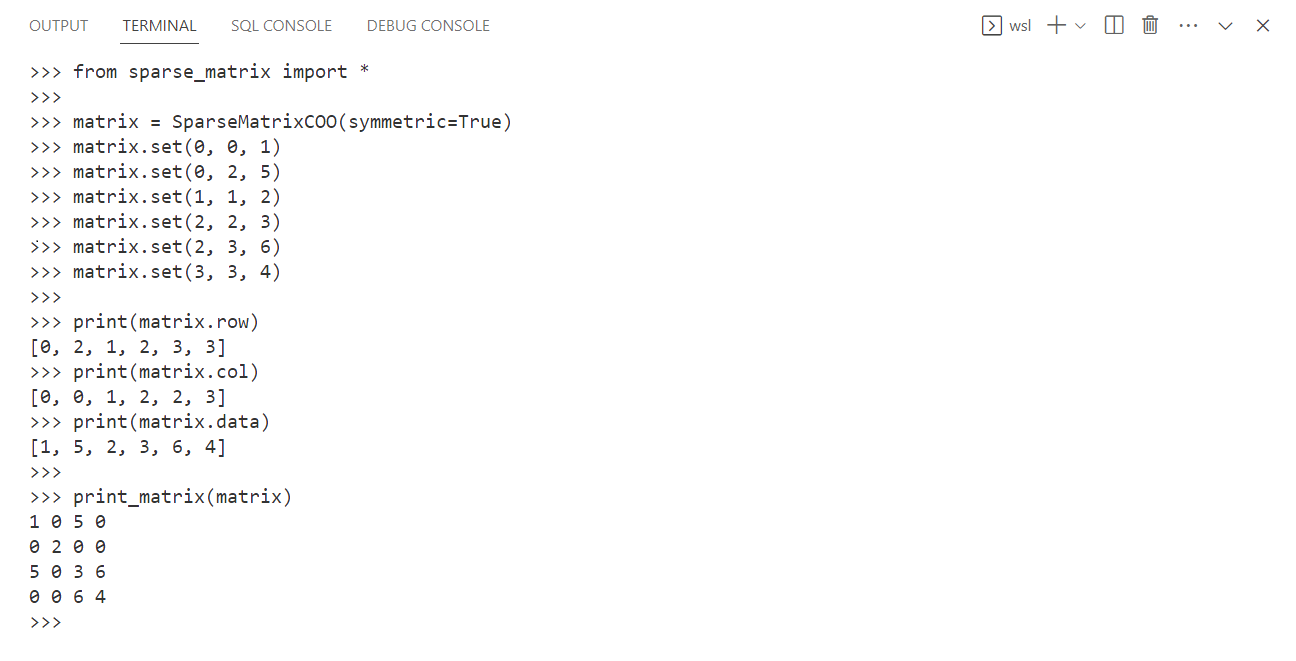
\includegraphics[width=0.95\textwidth]{img/sparse1.pdf} }
%     \caption{Инициализация матрицы}
% \end{figure}
После инициализации матрица переводится в сжатый разреженный строчный вид (\textbf{C}ompressed \textbf{S}parse \textbf{R}ow format),
и дальше сохраняет этот вид при всех последующих операциях с ней (при этом матрица становится неизменяемой).
% \begin{figure}[H]
%     \centering
%     \fbox{ 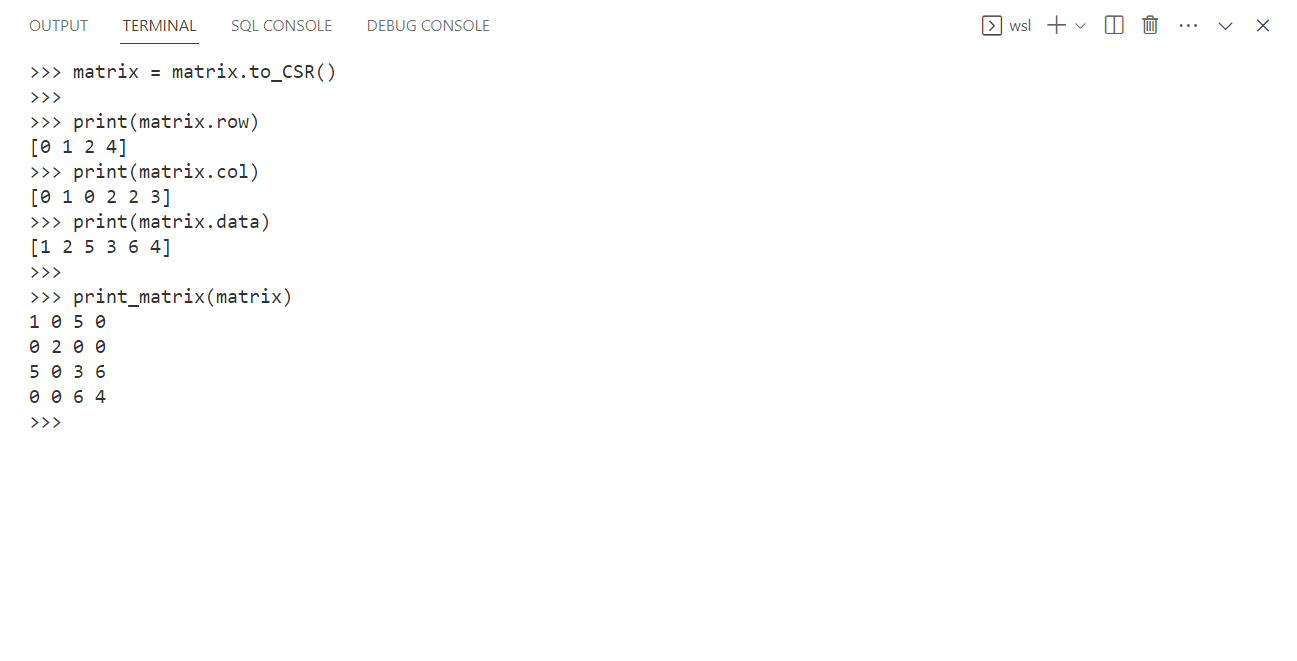
\includegraphics[width=0.95\textwidth]{img/sparse2.pdf} }
%     \caption{Перевод матрицы в новый вид}
% \end{figure}

  % \newpage
  % \section{Метод сопряженных градиентов}
  % Опишем метод решения следующей системы
\[ \vec{A}\vec{x} = \vec{b} \]
где матрица $\vec{A}$ симметричная и положительно определенная.
Возьмем произвольное начальное приближение $\vec{x}^{(0)}$.

\RestyleAlgo{tworuled}
\SetAlFnt{\normalsize}
\SetAlgoNoLine

\subsection{Явный метод}
\begin{algorithm*}[H]
    \DontPrintSemicolon

    $\vec{r}^{(0)} = \vec{b} - \vec{A} \vec{x}^{(0)}$\;
    $\vec{s}^{(1)} = \vec{r}^{(0)}$\;
    $\gamma = \sqrt{\left( \vec{b},\ \vec{b} \right)}$\;

    \For{$k = 1$ \KwTo $k_{max}$}{
        $\displaystyle
            \alpha_k = \frac{\left( \vec{r}^{(k-1)},\ \vec{r}^{(k-1)} \right)}{\left( \vec{A}\vec{s}^{(k)},\ \vec{s}^{(k)} \right)}
        $\;
        $\vec{x}^{(k)} = \vec{x}^{(k-1)} + \alpha_k \vec{s}^{(k)}$\;
        $\vec{r}^{(k)} = \vec{r}^{(k-1)} - \alpha_k \vec{s}^{(k-1)}$\;

        \If{$\sqrt{\left( \vec{r}^{(k)},\ \vec{r}^{(k)} \right)} < \gamma \varepsilon $}{
            \textbf{break}
        }

        $\displaystyle
            \beta_k = \frac{\left( \vec{r}^{(k)},\ \vec{r}^{(k)} \right)}{\left( \vec{r}^{(k-1)},\ \vec{r}^{(k-1)} \right)}
        $\;
        $\vec{s}^{(k+1)} = \vec{r}^{(k)} + \beta_k \vec{s}^{(k)}$\;
    }
\end{algorithm*}

\subsection{Неявный метод}
Неявный метод основан на идее предобуславливания. Выберем матрицу $\vec{B}$, симметричную и положительно определенную, такую, чтобы она была приблизительно равна матрице $\vec{A}$.
Возьмем $\vec{B} = \widetilde{\vec{L}} \widetilde{\vec{L}}^T$, где $\widetilde{\vec{L}} \widetilde{\vec{L}}^T$ -- неполное разложение
Холецкого для матрицы $\vec{A}$. Позже объясним, почему такой выбор матрицы $\vec{B}$ является удачным.

\begin{algorithm*}[H]
    \DontPrintSemicolon

    $\vec{r}^{(0)} = \vec{b} - \vec{A} \vec{x}^{(0)}$\;
    $\vec{B} \vec{w}^{(0)} = \vec{r}^{(0)}$\;
    $\vec{s}^{(1)} = \vec{w}^{(0)}$\;
    $\vec{B} \vec{g} = \vec{b}$\;
    $\gamma = \sqrt{\left( \vec{g},\ \vec{b} \right)}$\;

    \For{$k = 1$ \KwTo $k_{max}$}{
        $\displaystyle
            \alpha_k = \frac{\left( \vec{w}^{(k-1)},\ \vec{r}^{(k-1)} \right)}{\left( \vec{A}\vec{s}^{(k)},\ \vec{s}^{(k)} \right)}
        $\;
        $\vec{x}^{(k)} = \vec{x}^{(k-1)} + \alpha_k \vec{s}^{(k)}$\;
        $\vec{r}^{(k)} = \vec{r}^{(k-1)} - \alpha_k \vec{s}^{(k-1)}$\;
        $\vec{B}\vec{w}^{(k)} = \vec{r}^{(k)}$\;

        \If{$\sqrt{\left( \vec{w}^{(k)},\ \vec{r}^{(k)} \right)} < \gamma \varepsilon $}{
            \textbf{break}
        }

        $\displaystyle
            \beta_k = \frac{\left( \vec{w}^{(k)},\ \vec{r}^{(k)} \right)}{\left( \vec{w}^{(k-1)},\ \vec{r}^{(k-1)} \right)}
        $\;
        $\vec{s}^{(k+1)} = \vec{w}^{(k)} + \beta_k \vec{s}^{(k)}$\;
    }
\end{algorithm*}
\noindent Систему $\vec{B} \vec{w}^{(k)} = \vec{r}^{(k)}$ будем решать методом Гаусса. Выбирая $\vec{B} = \widetilde{\vec{L}}\widetilde{\vec{L}}^T$, остается только сделать два раза обратную
подстановку: $\widetilde{\vec{L}} \vec{z}^{(k)} = \vec{r}^{(k)}$ и $\widetilde{\vec{L}}^T \vec{w}^{(k)} = \vec{z}^{(k)}$.

\newpage
\begin{landscape}
\subsection{Пример работы алгоритма}
Рассмотрим следующий численный пример.
\begin{align*}
    \vec{A} &=
    \begin{pmatrix}
        3.56 & 1.27 & 0 & 1.20 & 0 & 0 & 0 & 0 & 0 \\
        1.27 & 5.82 & 1.58 & 0 & 1.81 & 0 & 0 & 0 & 0 \\
        0 & 1.58 & 3.31 & 1.33 & 0 & 1.83 & 0 & 0 & 0 \\
        1.20 & 0 & 1.33 & 5.08 & 1.20 & 0 & 1.87 & 0 & 0 \\
        0 & 1.81 & 0 & 1.20 & 5.67 & 1.94 & 0 & 1.24 & 0 \\
        0 & 0 & 1.83 & 0 & 1.94 & 3.44 & 1.78 & 0 & 1.25 \\
        0 & 0 & 0 & 1.87 & 0 & 1.78 & 4.03 & 1.70 & 0 \\
        0 & 0 & 0 & 0 & 1.24 & 0 & 1.70 & 5.29 & 1.64 \\
        0 & 0 & 0 & 0 & 0 & 1.25 & 0 & 1.64 & 5.64 \\
    \end{pmatrix}
    &
    \vec{x} &= \begin{pmatrix}
        1.95 \\ 1.98 \\ 1.88 \\ 1.41 \\ 1.37 \\ 1.16 \\ 1.99 \\ 1.46 \\ 1.94 \\
    \end{pmatrix}
    &
    \vec{b} &= \begin{pmatrix}
        11.17 \\ 19.44 \\ 13.34 \\ 17.37 \\ 17.11 \\ 16.07 \\ 15.21 \\ 16.02 \\ 14.81 \\
    \end{pmatrix} \\
\end{align*}
Задаимся нулевым начальным приближением и значением $\varepsilon = 0.01$. Обозначим сделанное количество итераций как $n$,
погрешность решения будем вычислять следующим образом.
\[
    \delta = \norm{\vec{x} - \tilde{\vec{x}}}_2
\]
Полученные решения для явного и неявного методов, соответственно, приведены ниже.
\[
    \tilde{\vec{x}}^T = \begin{pmatrix}
        1.92 & 2.01 & 1.85 & 1.39 & 1.36 & 1.14 & 2.05 & 1.46 & 1.95 \\
    \end{pmatrix},\quad n = 5,\quad \delta = 8.13 \cdot 10^{-2}
\]
\[
    \tilde{\vec{x}}^T = \begin{pmatrix}
        1.95 & 1.96 & 1.89 & 1.41 & 1.39 & 1.17 & 1.98 & 1.46 & 1.94 \\
    \end{pmatrix},\quad n = 4,\quad \delta = 2.97 \cdot 10^{-2}
\]
\end{landscape}

\newpage
\begin{landscape}
Также приведем разложение Холецкого для данного примера.
\[
    \widetilde{\vec{L}} =
    \begin{pmatrix}
        1.89 & 0 & 0 & 0 & 0 & 0 & 0 & 0 & 0 \\
        0.67 & 2.32 & 0 & 0 & 0 & 0 & 0 & 0 & 0 \\
        0 & 0.68 & 1.69 & 0 & 0 & 0 & 0 & 0 & 0 \\
        0.64 & 0 & 0.79 & 2.01 & 0 & 0 & 0 & 0 & 0 \\
        0 & 0.78 & 0 & 0.60 & 2.17 & 0 & 0 & 0 & 0 \\
        0 & 0 & 1.08 & 0 & 0.89 & 1.21 & 0 & 0 & 0 \\
        0 & 0 & 0 & 0.93 & 0 & 1.47 & 1.00 & 0 & 0 \\
        0 & 0 & 0 & 0 & 0.57 & 0 & 1.70 & 1.44 & 0 \\
        0 & 0 & 0 & 0 & 0 & 1.03 & 0 & 1.14 & 1.81 \\
    \end{pmatrix}
\]
\[
    \widetilde{\vec{L}} \widetilde{\vec{L}}^T =
    \begin{pmatrix}
        3.56 & 1.27 & 0.0 & 1.20 & 0.0 & 0.0 & 0.0 & 0.0 & 0.0 \\
        1.27 & 5.82 & 1.58 & 0.43 & 1.81 & 0.0 & 0.0 & 0.0 & 0.0 \\
        0.0 & 1.58 & 3.31 & 1.33 & 0.53 & 1.83 & 0.0 & 0.0 & 0.0 \\
        1.20 & 0.43 & 1.33 & 5.08 & 1.20 & 0.86 & 1.87 & 0.0 & 0.0 \\
        0.0 & 1.81 & 0.53 & 1.20 & 5.67 & 1.94 & 0.55 & 1.24 & 0.0 \\
        0.0 & 0.0 & 1.83 & 0.86 & 1.94 & 3.44 & 1.78 & 0.51 & 1.25 \\
        0.0 & 0.0 & 0.0 & 1.87 & 0.55 & 1.78 & 4.03 & 1.70 & 1.52 \\
        0.0 & 0.0 & 0.0 & 0.0 & 1.24 & 0.51 & 1.70 & 5.29 & 1.64 \\
        0.0 & 0.0 & 0.0 & 0.0 & 0.0 & 1.25 & 1.52 & 1.64 & 5.64 \\
    \end{pmatrix}
\]
\end{landscape}

Знаем, что матрица в диагональным преобладанием не будет плохо обусловленной.
Для того, чтобы продемонстрировать разную скорость сходимости двух методом,
выберем для тестов матрицу без явного диагонального преобладания. Матрицу заполним
случайными числами, размер матрицы -- 100. Зададим значение $\varepsilon = 10^{-5}$.
\begin{table}[H]
    \centering
    \begin{tabular}{*5c}
        \toprule
        \multirow[c]{2}{*}{\makecell{№\\теста}} & \multicolumn{2}{c}{Явный метод} & \multicolumn{2}{c}{Неявный метод} \\
        \cmidrule{2-5}
        & $n$ & $\delta$ & $n$ & $\delta$ \\
        \midrule
        1 & 38 & $1.87 \cdot 10^{-3}$ & 14 & $2.75 \cdot 10^{-4}$ \\
        2 & 37 & $4.92 \cdot 10^{-4}$ & 14 & $1.68 \cdot 10^{-4}$ \\
        3 & 35 & $4.12 \cdot 10^{-3}$ & 13 & $5.41 \cdot 10^{-4}$ \\
        \bottomrule
    \end{tabular}
\end{table}
\noindent Видим, что неявный метод сходится быстрее.

  % \newpage
  % \section{Тестирование построенной модели}
  % Для проверки построенной модели используем следующий набор пробных решений.
\begin{table}[H]
    \centering
    \begin{tabular}{*4c}
        \toprule
        \makecell{№\\теста} & $k_1(x, y)$ & $k_2(x, y)$ & $u(x, y)$ \\
        \midrule
        1 & $(x + y + 1)^2$ & $(x + y + 1)^3$ & $1$ \\
        2 & $x + y + 1$ & $x + y + 1$ & $2 x + 3 y + 1$ \\
        3 & $(x + y + 1)^2$ & $(x + y + 1)^2$ & $2 x + 3 y + 1$ \\
        4 & $(x + y + 1)^3$ & $(x + y + 1)^3$ & $2 x + 3 y + 1$ \\
        5 & $1$ & $1$ & $(2 x + 3 y + 1)^2$ \\
        6 & $x + y + 1$ & $x + y + 1$ & $(2 x + 3 y + 1)^2$ \\
        7 & $x + y + 1$ & $x + y + 1$ & $(2 x + 3 y + 1)^3$ \\
        8 & $\cos(x y) + 2$ & $\sin(x)\sin(y) + 2$ & $x \ln(y + 1)$ \\
        \bottomrule
    \end{tabular}
\end{table}
Для всех тестов определим следующие значения
\[ a = 0,\quad b = 1 \]
\[ c = 0,\quad d = 2 \]
\[ \chi_1 = 1,\quad \chi_3 = 3,\quad \chi_4 = 4 \]
Функция $f$, как и функции $g_1$, $g_2$, $g_3$, $g_4$, вычисляется программно с
использованием символьных вычислений и не приведена в описании теста.

Погрешность решения задачи будем вычислять тремя разными способами.
\begin{align*}
    \delta_1 &= \frac{\norm{\vec{x} - \tilde{\vec{x}}}_1}{\norm{\vec{x}}_1} &
    \delta_2 &= \frac{\norm{\vec{x} - \tilde{\vec{x}}}_2}{\norm{\vec{x}}_2} &
    \delta_3 &= \frac{\norm{\vec{x} - \tilde{\vec{x}}}_{\infty}}{\norm{\vec{x}}_{\infty}} \\
\end{align*}
Значение $\varepsilon$ для метода сопряженных градиентов равно $10^{-8}$.

\newpage
Тест №1 -- константный. Присутствует только ошибка округления.
\begin{table}[H]
	\centering
	\begin{tabular}{*6c}
		\toprule
		$N_x$ & $N_y$ & $n$ & $\delta_1$ & $\delta_2$ & $\delta_3$ \\
		\midrule
		2 & 2 & 7 & 1.22e-15 & 2.35e-15 & 6.44e-15 \\
		4 & 2 & 13 & 2.34e-11 & 4.84e-11 & 1.26e-10 \\
		2 & 4 & 12 & 1.56e-14 & 3.11e-14 & 9.48e-14 \\
		4 & 4 & 23 & 2.11e-12 & 3.95e-12 & 1.24e-11 \\
		8 & 4 & 47 & 2.40e-10 & 4.02e-10 & 1.28e-09 \\
		4 & 8 & 44 & 5.50e-11 & 1.09e-10 & 3.91e-10 \\
		8 & 8 & 72 & 2.10e-09 & 2.89e-09 & 1.00e-08 \\
		16 & 8 & 124 & 8.10e-09 & 1.07e-08 & 4.34e-08 \\
		8 & 16 & 118 & 1.56e-09 & 2.17e-09 & 9.56e-09 \\
		16 & 16 & 151 & 2.80e-09 & 4.10e-09 & 2.15e-08 \\
		32 & 16 & 247 & 8.38e-09 & 1.23e-08 & 9.07e-08 \\
		16 & 32 & 235 & 2.67e-09 & 4.65e-09 & 5.82e-08 \\
		32 & 32 & 294 & 7.84e-09 & 1.01e-08 & 3.86e-08 \\
		\bottomrule
	\end{tabular}
	\caption{Тест №1 (явный метод)}
\end{table}
\begin{table}[H]
	\centering
	\begin{tabular}{*6c}
		\toprule
		$N_x$ & $N_y$ & $n$ & $\delta_1$ & $\delta_2$ & $\delta_3$ \\
		\midrule
		2 & 2 & 5 & 8.64e-17 & 1.33e-16 & 3.33e-16 \\
		4 & 2 & 7 & 4.53e-10 & 8.68e-10 & 3.13e-09 \\
		2 & 4 & 7 & 7.49e-10 & 9.93e-10 & 2.09e-09 \\
		4 & 4 & 9 & 1.99e-09 & 2.74e-09 & 7.46e-09 \\
		8 & 4 & 11 & 3.87e-09 & 5.31e-09 & 1.67e-08 \\
		4 & 8 & 12 & 1.28e-10 & 1.70e-10 & 5.20e-10 \\
		8 & 8 & 15 & 1.02e-09 & 1.59e-09 & 5.04e-09 \\
		16 & 8 & 19 & 1.12e-09 & 1.65e-09 & 6.57e-09 \\
		8 & 16 & 20 & 4.73e-10 & 5.98e-10 & 1.70e-09 \\
		16 & 16 & 26 & 1.31e-09 & 2.05e-09 & 9.27e-09 \\
		32 & 16 & 33 & 2.90e-09 & 4.13e-09 & 1.76e-08 \\
		16 & 32 & 35 & 2.26e-09 & 3.34e-09 & 1.27e-08 \\
		32 & 32 & 47 & 6.73e-09 & 9.72e-09 & 3.67e-08 \\
		\bottomrule
	\end{tabular}
	\caption{Тест №1 (неявный метод)}
\end{table}

\newpage
Тест №2 -- линейный. Присутствует только ошибка округления.
\begin{table}[H]
	\centering
	\begin{tabular}{*6c}
		\toprule
		$N_x$ & $N_y$ & $n$ & $\delta_1$ & $\delta_2$ & $\delta_3$ \\
		\midrule
		2 & 2 & 7 & 4.05e-16 & 6.19e-16 & 8.88e-16 \\
		4 & 2 & 13 & 2.71e-11 & 4.68e-11 & 7.66e-11 \\
		2 & 4 & 11 & 3.08e-16 & 4.40e-16 & 6.91e-16 \\
		4 & 4 & 21 & 1.15e-10 & 2.03e-10 & 3.97e-10 \\
		8 & 4 & 43 & 6.25e-09 & 7.26e-09 & 1.01e-08 \\
		4 & 8 & 34 & 7.81e-10 & 1.09e-09 & 1.92e-09 \\
		8 & 8 & 53 & 7.59e-09 & 9.49e-09 & 2.11e-08 \\
		16 & 8 & 99 & 4.65e-09 & 5.88e-09 & 9.04e-09 \\
		8 & 16 & 65 & 1.88e-09 & 2.45e-09 & 6.74e-09 \\
		16 & 16 & 105 & 3.67e-09 & 4.57e-09 & 1.05e-08 \\
		32 & 16 & 196 & 1.11e-08 & 1.47e-08 & 3.09e-08 \\
		16 & 32 & 131 & 3.73e-09 & 4.28e-09 & 6.71e-09 \\
		32 & 32 & 208 & 8.67e-09 & 9.88e-09 & 2.30e-08 \\
		\bottomrule
	\end{tabular}
	\caption{Тест №2 (явный метод)}
\end{table}
\begin{table}[H]
	\centering
	\begin{tabular}{*6c}
		\toprule
		$N_x$ & $N_y$ & $n$ & $\delta_1$ & $\delta_2$ & $\delta_3$ \\
		\midrule
		2 & 2 & 5 & 5.43e-17 & 1.09e-16 & 1.97e-16 \\
		4 & 2 & 6 & 3.86e-10 & 4.45e-10 & 5.65e-10 \\
		2 & 4 & 7 & 7.82e-11 & 1.11e-10 & 1.64e-10 \\
		4 & 4 & 8 & 3.94e-09 & 4.93e-09 & 8.23e-09 \\
		8 & 4 & 10 & 4.51e-10 & 5.48e-10 & 9.80e-10 \\
		4 & 8 & 11 & 3.19e-10 & 3.91e-10 & 5.13e-10 \\
		8 & 8 & 14 & 1.39e-09 & 1.70e-09 & 3.02e-09 \\
		16 & 8 & 16 & 3.16e-09 & 3.94e-09 & 7.61e-09 \\
		8 & 16 & 18 & 1.04e-09 & 1.21e-09 & 1.76e-09 \\
		16 & 16 & 24 & 2.92e-09 & 3.68e-09 & 7.74e-09 \\
		32 & 16 & 29 & 4.89e-09 & 6.02e-09 & 1.03e-08 \\
		16 & 32 & 32 & 7.51e-09 & 9.51e-09 & 1.74e-08 \\
		32 & 32 & 44 & 6.04e-09 & 7.63e-09 & 1.49e-08 \\
		\bottomrule
	\end{tabular}
	\caption{Тест №2 (неявный метод)}
\end{table}

\newpage
Тест №3 -- линейный. Присутствует как ошибка округления, так и ошибка аппроксимации.
\begin{table}[H]
	\centering
	\begin{tabular}{*6c}
		\toprule
		$N_x$ & $N_y$ & $n$ & $\delta_1$ & $\delta_2$ & $\delta_3$ \\
		\midrule
		2 & 2 & 7 & 5.37e-03 & 7.88e-03 & 1.21e-02 \\
		4 & 2 & 13 & 5.02e-03 & 6.93e-03 & 9.76e-03 \\
		2 & 4 & 11 & 1.93e-03 & 2.96e-03 & 5.12e-03 \\
		4 & 4 & 22 & 1.27e-03 & 1.88e-03 & 3.38e-03 \\
		8 & 4 & 48 & 1.20e-03 & 1.71e-03 & 2.89e-03 \\
		4 & 8 & 39 & 4.65e-04 & 6.77e-04 & 1.33e-03 \\
		8 & 8 & 67 & 2.89e-04 & 4.26e-04 & 8.80e-04 \\
		16 & 8 & 132 & 2.70e-04 & 3.87e-04 & 7.70e-04 \\
		8 & 16 & 88 & 1.12e-04 & 1.59e-04 & 3.37e-04 \\
		16 & 16 & 138 & 6.74e-05 & 9.82e-05 & 2.23e-04 \\
		32 & 16 & 258 & 6.23e-05 & 8.87e-05 & 1.97e-04 \\
		16 & 32 & 168 & 2.73e-05 & 3.82e-05 & 8.45e-05 \\
		32 & 32 & 273 & 1.62e-05 & 2.34e-05 & 5.61e-05 \\
		\bottomrule
	\end{tabular}
	\caption{Тест №3 (явный метод)}
\end{table}
\begin{table}[H]
	\centering
	\begin{tabular}{*6c}
		\toprule
		$N_x$ & $N_y$ & $n$ & $\delta_1$ & $\delta_2$ & $\delta_3$ \\
		\midrule
		2 & 2 & 5 & 5.37e-03 & 7.88e-03 & 1.21e-02 \\
		4 & 2 & 6 & 5.02e-03 & 6.93e-03 & 9.76e-03 \\
		2 & 4 & 7 & 1.93e-03 & 2.96e-03 & 5.12e-03 \\
		4 & 4 & 9 & 1.27e-03 & 1.88e-03 & 3.38e-03 \\
		8 & 4 & 10 & 1.20e-03 & 1.71e-03 & 2.89e-03 \\
		4 & 8 & 11 & 4.65e-04 & 6.77e-04 & 1.33e-03 \\
		8 & 8 & 14 & 2.89e-04 & 4.26e-04 & 8.80e-04 \\
		16 & 8 & 17 & 2.70e-04 & 3.87e-04 & 7.70e-04 \\
		8 & 16 & 18 & 1.12e-04 & 1.59e-04 & 3.37e-04 \\
		16 & 16 & 24 & 6.74e-05 & 9.82e-05 & 2.23e-04 \\
		32 & 16 & 29 & 6.23e-05 & 8.87e-05 & 1.97e-04 \\
		16 & 32 & 32 & 2.73e-05 & 3.82e-05 & 8.45e-05 \\
		32 & 32 & 44 & 1.62e-05 & 2.34e-05 & 5.61e-05 \\
		\bottomrule
	\end{tabular}
	\caption{Тест №3 (неявный метод)}
\end{table}

\newpage
Тест №4 -- линейный. Присутствует как ошибка округления, так и ошибка аппроксимации.
\begin{table}[H]
	\centering
	\begin{tabular}{*6c}
		\toprule
		$N_x$ & $N_y$ & $n$ & $\delta_1$ & $\delta_2$ & $\delta_3$ \\
		\midrule
		2 & 2 & 7 & 1.60e-02 & 2.34e-02 & 3.57e-02 \\
		4 & 2 & 15 & 1.53e-02 & 2.11e-02 & 2.98e-02 \\
		2 & 4 & 11 & 5.66e-03 & 8.71e-03 & 1.51e-02 \\
		4 & 4 & 24 & 3.90e-03 & 5.73e-03 & 1.02e-02 \\
		8 & 4 & 53 & 3.73e-03 & 5.28e-03 & 8.86e-03 \\
		4 & 8 & 44 & 1.36e-03 & 2.01e-03 & 4.01e-03 \\
		8 & 8 & 87 & 8.94e-04 & 1.31e-03 & 2.68e-03 \\
		16 & 8 & 167 & 8.48e-04 & 1.20e-03 & 2.36e-03 \\
		8 & 16 & 120 & 3.25e-04 & 4.70e-04 & 1.02e-03 \\
		16 & 16 & 195 & 2.09e-04 & 3.01e-04 & 6.80e-04 \\
		32 & 16 & 360 & 1.96e-04 & 2.76e-04 & 6.04e-04 \\
		16 & 32 & 241 & 7.90e-05 & 1.13e-04 & 2.56e-04 \\
		32 & 32 & 380 & 5.00e-05 & 7.16e-05 & 1.71e-04 \\
		\bottomrule
	\end{tabular}
	\caption{Тест №4 (явный метод)}
\end{table}
\begin{table}[H]
	\centering
	\begin{tabular}{*6c}
		\toprule
		$N_x$ & $N_y$ & $n$ & $\delta_1$ & $\delta_2$ & $\delta_3$ \\
		\midrule
		2 & 2 & 5 & 1.60e-02 & 2.34e-02 & 3.57e-02 \\
		4 & 2 & 6 & 1.53e-02 & 2.11e-02 & 2.98e-02 \\
		2 & 4 & 7 & 5.66e-03 & 8.71e-03 & 1.51e-02 \\
		4 & 4 & 9 & 3.90e-03 & 5.73e-03 & 1.02e-02 \\
		8 & 4 & 10 & 3.73e-03 & 5.28e-03 & 8.86e-03 \\
		4 & 8 & 11 & 1.36e-03 & 2.01e-03 & 4.01e-03 \\
		8 & 8 & 14 & 8.94e-04 & 1.31e-03 & 2.68e-03 \\
		16 & 8 & 16 & 8.48e-04 & 1.20e-03 & 2.36e-03 \\
		8 & 16 & 18 & 3.25e-04 & 4.70e-04 & 1.02e-03 \\
		16 & 16 & 24 & 2.09e-04 & 3.01e-04 & 6.80e-04 \\
		32 & 16 & 29 & 1.96e-04 & 2.76e-04 & 6.04e-04 \\
		16 & 32 & 31 & 7.90e-05 & 1.13e-04 & 2.56e-04 \\
		32 & 32 & 43 & 5.00e-05 & 7.16e-05 & 1.71e-04 \\
		\bottomrule
	\end{tabular}
	\caption{Тест №4 (неявный метод)}
\end{table}

\newpage
Тест №5 -- полиномиальный. Присутствует только ошибка округления.
\begin{table}[H]
	\centering
	\begin{tabular}{*6c}
		\toprule
		$N_x$ & $N_y$ & $n$ & $\delta_1$ & $\delta_2$ & $\delta_3$ \\
		\midrule
		2 & 2 & 7 & 8.80e-17 & 1.26e-16 & 1.75e-16 \\
		4 & 2 & 13 & 1.26e-13 & 1.85e-13 & 2.35e-13 \\
		2 & 4 & 11 & 2.21e-16 & 2.30e-16 & 1.75e-16 \\
		4 & 4 & 21 & 1.02e-14 & 1.17e-14 & 1.24e-14 \\
		8 & 4 & 37 & 3.46e-09 & 3.57e-09 & 4.31e-09 \\
		4 & 8 & 26 & 4.78e-09 & 5.54e-09 & 8.19e-09 \\
		8 & 8 & 43 & 4.88e-09 & 5.06e-09 & 6.56e-09 \\
		16 & 8 & 81 & 6.43e-09 & 6.76e-09 & 1.05e-08 \\
		8 & 16 & 54 & 2.22e-09 & 2.71e-09 & 7.02e-09 \\
		16 & 16 & 83 & 8.25e-09 & 8.74e-09 & 1.19e-08 \\
		32 & 16 & 146 & 9.20e-09 & 1.01e-08 & 1.36e-08 \\
		16 & 32 & 105 & 4.99e-09 & 6.05e-09 & 9.70e-09 \\
		32 & 32 & 163 & 9.63e-09 & 1.12e-08 & 1.92e-08 \\
		\bottomrule
	\end{tabular}
	\caption{Тест №5 (явный метод)}
\end{table}
\begin{table}[H]
	\centering
	\begin{tabular}{*6c}
		\toprule
		$N_x$ & $N_y$ & $n$ & $\delta_1$ & $\delta_2$ & $\delta_3$ \\
		\midrule
		2 & 2 & 5 & 1.41e-16 & 1.53e-16 & 1.75e-16 \\
		4 & 2 & 6 & 1.81e-10 & 1.80e-10 & 2.31e-10 \\
		2 & 4 & 6 & 1.10e-09 & 1.37e-09 & 1.87e-09 \\
		4 & 4 & 8 & 2.60e-09 & 2.58e-09 & 2.48e-09 \\
		8 & 4 & 9 & 3.87e-09 & 3.70e-09 & 3.94e-09 \\
		4 & 8 & 10 & 9.67e-10 & 1.07e-09 & 1.16e-09 \\
		8 & 8 & 13 & 4.84e-09 & 5.13e-09 & 6.05e-09 \\
		16 & 8 & 15 & 6.37e-09 & 6.34e-09 & 6.52e-09 \\
		8 & 16 & 17 & 1.82e-09 & 1.95e-09 & 2.46e-09 \\
		16 & 16 & 23 & 7.17e-09 & 7.69e-09 & 1.08e-08 \\
		32 & 16 & 28 & 8.27e-09 & 8.44e-09 & 1.12e-08 \\
		16 & 32 & 31 & 8.83e-09 & 9.43e-09 & 1.10e-08 \\
		32 & 32 & 43 & 5.85e-09 & 6.33e-09 & 8.54e-09 \\
		\bottomrule
	\end{tabular}
	\caption{Тест №5 (неявный метод)}
\end{table}

\newpage
Тест №6 -- полиномиальный. Присутствует как ошибка округления, так и ошибка аппроксимации.
\begin{table}[H]
	\centering
	\begin{tabular}{*6c}
		\toprule
		$N_x$ & $N_y$ & $n$ & $\delta_1$ & $\delta_2$ & $\delta_3$ \\
		\midrule
		2 & 2 & 7 & 7.61e-03 & 8.62e-03 & 9.27e-03 \\
		4 & 2 & 13 & 7.80e-03 & 8.50e-03 & 8.32e-03 \\
		2 & 4 & 11 & 2.50e-03 & 2.99e-03 & 3.54e-03 \\
		4 & 4 & 21 & 1.98e-03 & 2.27e-03 & 2.55e-03 \\
		8 & 4 & 44 & 1.98e-03 & 2.22e-03 & 2.38e-03 \\
		4 & 8 & 33 & 6.35e-04 & 7.40e-04 & 9.09e-04 \\
		8 & 8 & 55 & 4.71e-04 & 5.45e-04 & 6.63e-04 \\
		16 & 8 & 99 & 4.64e-04 & 5.27e-04 & 6.17e-04 \\
		8 & 16 & 65 & 1.57e-04 & 1.81e-04 & 2.29e-04 \\
		16 & 16 & 105 & 1.13e-04 & 1.30e-04 & 1.68e-04 \\
		32 & 16 & 196 & 1.10e-04 & 1.25e-04 & 1.56e-04 \\
		16 & 32 & 131 & 3.90e-05 & 4.46e-05 & 5.73e-05 \\
		32 & 32 & 208 & 2.74e-05 & 3.16e-05 & 4.21e-05 \\
		\bottomrule
	\end{tabular}
	\caption{Тест №6 (явный метод)}
\end{table}
\begin{table}[H]
	\centering
	\begin{tabular}{*6c}
		\toprule
		$N_x$ & $N_y$ & $n$ & $\delta_1$ & $\delta_2$ & $\delta_3$ \\
		\midrule
		2 & 2 & 5 & 7.61e-03 & 8.62e-03 & 9.27e-03 \\
		4 & 2 & 6 & 7.80e-03 & 8.50e-03 & 8.32e-03 \\
		2 & 4 & 7 & 2.50e-03 & 2.99e-03 & 3.54e-03 \\
		4 & 4 & 8 & 1.98e-03 & 2.27e-03 & 2.55e-03 \\
		8 & 4 & 10 & 1.98e-03 & 2.22e-03 & 2.38e-03 \\
		4 & 8 & 11 & 6.35e-04 & 7.40e-04 & 9.09e-04 \\
		8 & 8 & 14 & 4.71e-04 & 5.45e-04 & 6.63e-04 \\
		16 & 8 & 16 & 4.64e-04 & 5.27e-04 & 6.17e-04 \\
		8 & 16 & 18 & 1.57e-04 & 1.81e-04 & 2.29e-04 \\
		16 & 16 & 24 & 1.13e-04 & 1.30e-04 & 1.68e-04 \\
		32 & 16 & 29 & 1.10e-04 & 1.25e-04 & 1.56e-04 \\
		16 & 32 & 32 & 3.90e-05 & 4.46e-05 & 5.73e-05 \\
		32 & 32 & 44 & 2.74e-05 & 3.16e-05 & 4.21e-05 \\
		\bottomrule
	\end{tabular}
	\caption{Тест №6 (неявный метод)}
\end{table}

\newpage
Тест №7 -- полиномиальный. Присутствует как ошибка округления, так и ошибка аппроксимации.
\begin{table}[H]
	\centering
	\begin{tabular}{*6c}
		\toprule
		$N_x$ & $N_y$ & $n$ & $\delta_1$ & $\delta_2$ & $\delta_3$ \\
		\midrule
		2 & 2 & 7 & 2.51e-02 & 2.39e-02 & 1.84e-02 \\
		4 & 2 & 13 & 2.81e-02 & 2.68e-02 & 2.20e-02 \\
		2 & 4 & 11 & 7.74e-03 & 7.27e-03 & 4.96e-03 \\
		4 & 4 & 21 & 7.43e-03 & 7.09e-03 & 6.00e-03 \\
		8 & 4 & 44 & 7.81e-03 & 7.52e-03 & 6.43e-03 \\
		4 & 8 & 33 & 2.15e-03 & 1.99e-03 & 1.29e-03 \\
		8 & 8 & 55 & 1.88e-03 & 1.81e-03 & 1.57e-03 \\
		16 & 8 & 99 & 1.93e-03 & 1.88e-03 & 1.67e-03 \\
		8 & 16 & 64 & 5.57e-04 & 5.09e-04 & 3.24e-04 \\
		16 & 16 & 105 & 4.66e-04 & 4.49e-04 & 3.96e-04 \\
		32 & 16 & 196 & 4.70e-04 & 4.60e-04 & 4.20e-04 \\
		16 & 32 & 131 & 1.41e-04 & 1.28e-04 & 8.13e-05 \\
		32 & 32 & 207 & 1.15e-04 & 1.11e-04 & 9.93e-05 \\
		\bottomrule
	\end{tabular}
	\caption{Тест №7 (явный метод)}
\end{table}
\begin{table}[H]
	\centering
	\begin{tabular}{*6c}
		\toprule
		$N_x$ & $N_y$ & $n$ & $\delta_1$ & $\delta_2$ & $\delta_3$ \\
		\midrule
		2 & 2 & 4 & 2.51e-02 & 2.39e-02 & 1.84e-02 \\
		4 & 2 & 6 & 2.81e-02 & 2.68e-02 & 2.20e-02 \\
		2 & 4 & 6 & 7.74e-03 & 7.27e-03 & 4.96e-03 \\
		4 & 4 & 8 & 7.43e-03 & 7.09e-03 & 6.00e-03 \\
		8 & 4 & 10 & 7.81e-03 & 7.52e-03 & 6.43e-03 \\
		4 & 8 & 11 & 2.15e-03 & 1.99e-03 & 1.29e-03 \\
		8 & 8 & 14 & 1.88e-03 & 1.81e-03 & 1.57e-03 \\
		16 & 8 & 17 & 1.93e-03 & 1.88e-03 & 1.67e-03 \\
		8 & 16 & 18 & 5.57e-04 & 5.09e-04 & 3.24e-04 \\
		16 & 16 & 24 & 4.66e-04 & 4.49e-04 & 3.96e-04 \\
		32 & 16 & 30 & 4.70e-04 & 4.60e-04 & 4.20e-04 \\
		16 & 32 & 32 & 1.41e-04 & 1.28e-04 & 8.13e-05 \\
		32 & 32 & 45 & 1.15e-04 & 1.11e-04 & 9.93e-05 \\
		\bottomrule
	\end{tabular}
	\caption{Тест №7 (неявный метод)}
\end{table}

\newpage
Тест №8 добавлен для дополнительной проверки написанной модели.
Присутствует как ошибка округления, так и ошибка аппроксимации.
\begin{table}[H]
	\centering
	\begin{tabular}{*6c}
		\toprule
		$N_x$ & $N_y$ & $n$ & $\delta_1$ & $\delta_2$ & $\delta_3$ \\
		\midrule
		2 & 2 & 7 & 1.79e-02 & 1.57e-02 & 1.58e-02 \\
		4 & 2 & 13 & 1.31e-02 & 1.26e-02 & 1.10e-02 \\
		2 & 4 & 11 & 1.07e-02 & 1.12e-02 & 1.24e-02 \\
		4 & 4 & 21 & 4.37e-03 & 4.40e-03 & 4.07e-03 \\
		8 & 4 & 43 & 3.28e-03 & 3.92e-03 & 4.27e-03 \\
		4 & 8 & 31 & 2.59e-03 & 2.75e-03 & 3.24e-03 \\
		8 & 8 & 51 & 1.06e-03 & 1.11e-03 & 1.29e-03 \\
		16 & 8 & 95 & 7.41e-04 & 9.68e-04 & 1.32e-03 \\
		8 & 16 & 58 & 6.30e-04 & 6.74e-04 & 8.28e-04 \\
		16 & 16 & 94 & 2.52e-04 & 2.66e-04 & 3.52e-04 \\
		32 & 16 & 173 & 1.69e-04 & 2.23e-04 & 3.59e-04 \\
		16 & 32 & 113 & 1.55e-04 & 1.66e-04 & 2.07e-04 \\
		32 & 32 & 180 & 6.05e-05 & 6.40e-05 & 9.02e-05 \\
		\bottomrule
	\end{tabular}
	\caption{Тест №8 (явный метод)}
\end{table}
\begin{table}[H]
	\centering
	\begin{tabular}{*6c}
		\toprule
		$N_x$ & $N_y$ & $n$ & $\delta_1$ & $\delta_2$ & $\delta_3$ \\
		\midrule
		2 & 2 & 5 & 1.79e-02 & 1.57e-02 & 1.58e-02 \\
		4 & 2 & 6 & 1.31e-02 & 1.26e-02 & 1.10e-02 \\
		2 & 4 & 7 & 1.07e-02 & 1.12e-02 & 1.24e-02 \\
		4 & 4 & 9 & 4.37e-03 & 4.40e-03 & 4.07e-03 \\
		8 & 4 & 10 & 3.28e-03 & 3.92e-03 & 4.27e-03 \\
		4 & 8 & 11 & 2.59e-03 & 2.75e-03 & 3.24e-03 \\
		8 & 8 & 14 & 1.06e-03 & 1.11e-03 & 1.29e-03 \\
		16 & 8 & 16 & 7.41e-04 & 9.68e-04 & 1.32e-03 \\
		8 & 16 & 18 & 6.30e-04 & 6.74e-04 & 8.28e-04 \\
		16 & 16 & 24 & 2.52e-04 & 2.66e-04 & 3.52e-04 \\
		32 & 16 & 28 & 1.69e-04 & 2.23e-04 & 3.59e-04 \\
		16 & 32 & 33 & 1.55e-04 & 1.66e-04 & 2.07e-04 \\
		32 & 32 & 44 & 6.05e-05 & 6.40e-05 & 9.02e-05 \\
		\bottomrule
	\end{tabular}
	\caption{Тест №8 (неявный метод)}
\end{table}

\newpage
Дадим общую информацию по всем тестам.
\begin{itemize}
	\item Неявный метод показывает гораздо большую скорость
	сходимости.
	\item При наличии ошибки аппроксимации с увеличением числа
	разбиений в \textit{два} раза погрешность уменьшается примерно в
	\textit{четыре} раза: значение может быть болеше или меньше в зависимости от
	способа вычисления погрешности, но приближается к четырем с
	увеличением числа разбиений до достаточных величин.
	\item Напомним, что одномерная нуменация неизвестных велась
	вдоль оси $x$, поэтому в случае, когда число неизвестных
	вдоль выбранного направления больше, то есть $N_x > N_y$,
	можем наблюдать увеличение числа итераций метода, необходимых
	для получения решения.
\end{itemize}

  % \newpage
  % \section*{Заключение}\label{conclusion}
  % \addcontentsline{toc}{section}{\nameref{conclusion}}
  % В рамках данной курсовой работы было проведено практическое применение знаний в области
разработки программного обеспечения для моделирования стационарных процессов, с примером
процессов теплопроводности. Были изучены методы построения дискретных моделей для решения
задач моделирования стационарных процессов, а также проведена практика в разработке тестовых
примеров для отладки программ на основе метода пробных решений.

В ходе работы была разработана программа на алгоритмическом языке для решения конкретной
задачи моделирования стационарных процессов теплопроводности. Была проведена отладка программы
и решение конкретной задачи. Также было выполнено экспериментальное исследование точностных и
временных характеристик программного обеспечения. Результаты моделирования были представлены в
виде таблиц.

  % \newpage
  % \section*{Приложение. Текст программы}\label{appendix-listing}
  % \addcontentsline{toc}{section}{\nameref{appendix-listing}}

  % \lstinputlisting[caption={main.py}]{lst/main.py}
  % \lstinputlisting[caption={model.py}]{lst/model.py}
  % \lstinputlisting[caption={sparse\_matrix.py}]{lst/sparse\_matrix.py}\
  % \lstinputlisting[caption={linalg.py}]{lst/linalg.py}
  % \lstinputlisting[caption={grid.py}]{lst/grid.py}
  % \lstinputlisting[caption={utils.py}]{lst/utils.py}

\end{document}
